% ============================================================================
% Deep Surrogate Models & Gaussian Processes
% University of Geneva
% April 20--23 & May 4--7, 2026
% Duration: 90 minutes
% ============================================================================

\documentclass[aspectratio=169,11pt]{beamer}

% ---------- Theme and colors ----------
\usecolortheme{dove}
\setbeamertemplate{navigation symbols}{}
\setbeamertemplate{footline}{%
  \hfill\usebeamerfont{page number in head/foot}%
  \usebeamercolor[fg]{normal text}%
  \insertframenumber\,/\,\inserttotalframenumber\kern1em\vskip4pt}
\setbeamerfont{frametitle}{size=\huge}

% ---------- Packages ----------
\usepackage[utf8]{inputenc}
\usepackage[T1]{fontenc}
\usepackage{amsmath,amssymb,amsfonts}
\usepackage{bm}
\usepackage{graphicx}
\usepackage{tikz}
\usetikzlibrary{shapes,arrows.meta,positioning,calc,fit,backgrounds,patterns,decorations.pathreplacing}
\usepackage{pgfplots}
\pgfplotsset{compat=1.18}
\usepackage{booktabs}
\usepackage{hyperref}
\usepackage{multicol}
\usepackage{xcolor}
\usepackage{algorithm}
\usepackage{algorithmic}
\usepackage{listings}
\usepackage{pifont}

% ---------- Listings style for Python ----------
\lstset{
    language=Python,
    basicstyle=\small\ttfamily,
    keywordstyle=\color{uzhblue}\bfseries,
    commentstyle=\color{uzhgreydark}\itshape,
    stringstyle=\color{darkgreen},
    showstringspaces=false,
    breaklines=true,
    frame=none,
    xleftmargin=0pt,
    aboveskip=4pt,
    belowskip=4pt,
    escapeinside={(*@}{@*)},
}

% ---------- Custom colors ----------
\definecolor{uzhblue}{rgb}{0,0,0.5}
\definecolor{uzhgreylight}{RGB}{236,238,241}
\definecolor{uzhgreydark}{RGB}{81,86,94}
\definecolor{harvardcrimson}{RGB}{153,0,0}
\definecolor{unil@blue}{RGB}{0,140,204}
\definecolor{unil@black}{RGB}{35,31,32}
\definecolor{darkgreen}{RGB}{0,100,0}
\definecolor{darkred}{RGB}{139,0,0}
\definecolor{softblue}{RGB}{70,130,180}
\definecolor{softorange}{RGB}{230,159,0}
\definecolor{softgreen}{RGB}{0,158,115}

% ---------- Set beamer colors ----------
\setbeamercolor{frametitle}{bg=uzhgreylight, fg=uzhblue}
\setbeamercolor{title}{fg=uzhblue}
\setbeamercolor{structure}{fg=uzhblue}
\setbeamercolor{block title}{bg=unil@blue, fg=white}
\setbeamercolor{block body}{bg=uzhgreylight}
\setbeamercolor{block title alerted}{bg=darkred,fg=white}
\setbeamercolor{block body alerted}{bg=red!5}
\setbeamercolor{block title example}{bg=darkgreen,fg=white}
\setbeamercolor{block body example}{bg=green!5}
\setbeamercolor{item}{fg=unil@black}
\setbeamercolor{normal text}{fg=unil@black}

% ---------- Emphasis and hyperlinks ----------
\newcommand{\emphc}[1]{\textcolor{harvardcrimson}{#1}}
\hypersetup{colorlinks,linkcolor=harvardcrimson,urlcolor=harvardcrimson}

% ---------- Math commands ----------
\newcommand{\x}{\bm{x}}
\newcommand{\w}{\bm{w}}
\newcommand{\bb}{\bm{b}}
\newcommand{\z}{\bm{z}}
\newcommand{\W}{\bm{W}}
\newcommand{\X}{\bm{X}}
\renewcommand{\a}{\bm{a}}
\newcommand{\R}{\mathbb{R}}
\newcommand{\E}[1]{\mathbb{E}\!\left[#1\right]}
\DeclareMathOperator*{\argmin}{arg\,min}
\DeclareMathOperator*{\argmax}{arg\,max}

% ---------- Title ----------
\title[Deep Learning -- Geneva 2026]%
{Deep Learning for Economics and Finance}
\subtitle{Deep surrogates, GPs, Bayesian active learning, deep kernels, GP-VFI, active subspaces}
\author{Simon Scheidegger}
\institute[HEC Lausanne]{HEC, University of Lausanne}
\date{University of Geneva\\April 20--23 \& May 4--7, 2026}

\begin{document}

% --- Exercise pause badge ---
\newcommand{\exercisepause}{%
  \tikz[baseline=(X.base)]{\node[fill=darkgreen!80!black, text=white,
  rounded corners=2pt, inner sep=3pt, font=\scriptsize\bfseries](X){PAUSE --- 5 min};}}

% ============================================================================
% PART 0: TITLE & OUTLINE
% ============================================================================

% --- Slide 1: Title ---
{\setbeamercolor{background canvas}{bg=uzhgreylight}
\begin{frame}
\titlepage
\vspace{-0.4cm}
\begin{center}
{\footnotesize Based on: Chen, Didisheim \& Scheidegger (2026), \emph{J.\ Financial Economics}; Friedl et al.\ (2023); K\"ubler, Scheidegger \& Surbek (2026, forthcoming in \emph{JPE Macroeconomics})}\\[4pt]
{\footnotesize Materials: \url{https://github.com/sischei/Deep_Learning_for_Solving_And_Estimating_Dynamic_Economic_Models}}
\end{center}
\end{frame}
}

% --- Slide 2: Outline ---
\begin{frame}{Outline}
\tableofcontents
\end{frame}

% ============================================================================
% PART I: DEEP SURROGATE MODELS
% ============================================================================
\section{Deep Surrogate Models}

% --- Slide 3: Motivation ---
\begin{frame}{Motivation: Why Surrogates?}
\begin{block}{The computational bottleneck}
Economic \& financial models are expensive to evaluate:
\begin{itemize}
  \item Solving Bellman equations / dynamic programming (DEQNs)
  \item PDE-based models (HJB, Black--Scholes for exotics)
  \item Monte Carlo simulations for risk measures
\end{itemize}
\end{block}

\vspace{0.3cm}
\begin{alertblock}{Key insight}
\emphc{We know the true model} --- we can generate \emph{unlimited} training data by solving the model on a design of experiments.
\end{alertblock}

\vspace{0.3cm}
\textbf{Goal:} Build a \emphc{surrogate} $\phi(\cdot\,|\,\theta_{NN})$ that approximates $f(\cdot)$ but evaluates \emph{orders of magnitude faster}.
\end{frame}

% --- Slide 4: Look-up Tables to Neural Networks ---
\begin{frame}{Look-up Tables $\to$ Neural Networks}
\begin{columns}[T]
\begin{column}{0.42\textwidth}
\textbf{Traditional:} pre-compute \& interpolate.\\[2pt]
\begin{center}
\footnotesize
\begin{tabular}{cc}
\toprule
$x$ & $\Phi(x)$ \\
\midrule
$-2.0$ & $0.0228$ \\
$-1.0$ & $0.1587$ \\
$\phantom{-}0.0$ & $0.5000$ \\
$\phantom{-}1.0$ & $0.8413$ \\
$\phantom{-}2.0$ & $0.9772$ \\
\bottomrule
\end{tabular}
\end{center}
\vspace{2pt}
{\footnotesize Example: standard normal CDF table.}
\end{column}

\begin{column}{0.55\textwidth}
\textbf{21st-century look-up table:}\\[2pt]
A neural network memorizes $\x \mapsto y$:
\[
\phi(\x_t\,|\,\theta_{NN}) \approx y_t = f(\x_t)
\]
\vspace{-4pt}
\begin{center}
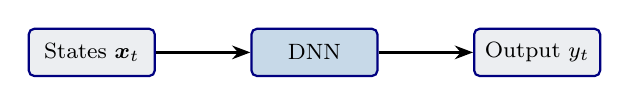
\begin{tikzpicture}[
    mlstep/.style={rectangle, draw=uzhblue, fill=uzhgreylight,
        minimum width=1.6cm, minimum height=0.6cm, font=\footnotesize,
        rounded corners=2pt, thick},
    >=Stealth
]
\node[mlstep] (input) {States $\x_t$};
\node[mlstep, right=1.2cm of input, fill=softblue!30] (dnn) {DNN};
\node[mlstep, right=1.2cm of dnn] (output) {Output $y_t$};
\draw[->, thick] (input) -- (dnn);
\draw[->, thick] (dnn) -- (output);
\end{tikzpicture}
\end{center}
\vspace{2pt}
{\footnotesize \emphc{Continuous}, \emphc{differentiable}, works in \emphc{any dimension}.}
\end{column}
\end{columns}
\end{frame}

% --- Slide 5: Pseudo-States ---
\begin{frame}{Pseudo-States: The Key Idea}
\begin{block}{Core insight (Chen, Didisheim \& Scheidegger 2026)}
Treat model parameters $\theta$ as \emphc{extra state variables}:
\vspace{-2pt}
\[
\tilde{\x} = \bigl(\underbrace{s_1,\dots,s_n}_{\text{states}},\;
\underbrace{h_1,\dots,h_h}_{\text{hidden}},\;
\underbrace{\theta_1,\dots,\theta_p}_{\text{parameters}}\bigr)
\in \R^{d}, \quad d = n + h + p.
\]
\vspace{-6pt}
\end{block}

\vspace{-0.1cm}
\begin{center}
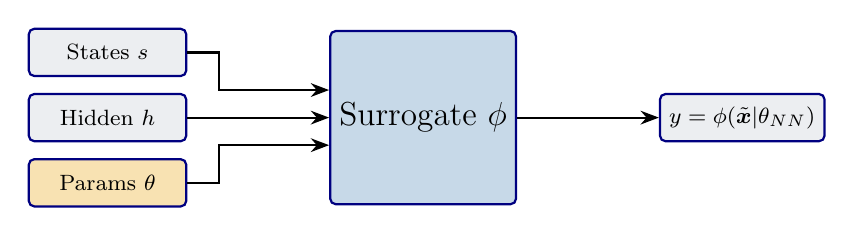
\begin{tikzpicture}[
    mlstep/.style={rectangle, draw=uzhblue, fill=uzhgreylight,
        minimum width=2cm, minimum height=0.6cm, font=\footnotesize,
        rounded corners=2pt, thick},
    >=Stealth
]
\node[mlstep] (states) {States $s$};
\node[mlstep, below=0.2cm of states] (hidden) {Hidden $h$};
\node[mlstep, below=0.2cm of hidden, fill=softorange!30] (params) {Params $\theta$};

\node[mlstep, right=1.8cm of hidden, fill=softblue!30,
      minimum width=2.2cm, minimum height=2.2cm] (surr) {\large Surrogate $\phi$};

\node[mlstep, right=1.8cm of surr] (output) {$y = \phi(\tilde{\x}|\theta_{NN})$};

\draw[->, thick] (states.east) -- ++(0.4,0) |- ([yshift=0.35cm]surr.west);
\draw[->, thick] (hidden.east) -- (surr.west);
\draw[->, thick] (params.east) -- ++(0.4,0) |- ([yshift=-0.35cm]surr.west);
\draw[->, thick] (surr) -- (output);
\end{tikzpicture}
\end{center}

\vspace{0.1cm}
Solve the model \emphc{once} over the full augmented space $\Rightarrow$ instant evaluation for \emph{any} parameter configuration.
\end{frame}

% --- Slide 6: Building the Surrogate ---
\begin{frame}{Building the Surrogate}
\begin{enumerate}
  \item \textbf{Design:} Draw $\tilde{\x}_i$ uniformly from $[\underline{x},\bar{x}]^d$, \quad $i = 1,\dots,m$.
  \item \textbf{Label:} Compute $y_i = f(\tilde{\x}_i)$ using the expensive model.
  \item \textbf{Train:} Minimize the empirical risk:
  \[
  \hat{\theta}_{NN} = \argmin_{\theta_{NN}} \frac{1}{m}\sum_{i=1}^{m}
  \bigl|\phi(\tilde{\x}_i\,|\,\theta_{NN}) - y_i\bigr|^2.
  \]
  \item \textbf{Validate:} On a held-out test set, compute max / mean absolute error.
\end{enumerate}

\vspace{0.4cm}
\begin{block}{Remark}
Since we can generate \emph{unlimited} data from the true model, the training set can be made as large as needed $\Rightarrow$ \emphc{no overfitting risk} in the traditional sense.
\end{block}
\end{frame}

% --- Slide 7: Why Surrogates Are Different ---
\begin{frame}[shrink=4]{Why Surrogates $\neq$ Standard ML}
\begin{columns}[T]
\begin{column}{0.48\textwidth}
\textbf{Standard supervised learning:}
\begin{itemize}
  \item Data is \emph{scarce} and noisy
  \item Overfitting is a major concern
  \item Regularization, early stopping, cross-validation
  \item Small learning rates, careful tuning
\end{itemize}
\end{column}
\begin{column}{0.48\textwidth}
\textbf{Surrogate modeling:}
\begin{itemize}
  \item Data is \emphc{unlimited} (we own the model)
  \item Labels are \emphc{exact} (or noise-free)
  \item Can use large epochs, aggressive LR
  \item Focus on \emph{approximation error}, not generalization
\end{itemize}
\end{column}
\end{columns}

\vspace{0.5cm}
\begin{block}{Once trained}
\begin{itemize}
  \item \emphc{Highly accurate} (errors $< 10^{-4}$ relative)
  \item \emphc{Orders of magnitude faster} than the original model
  \item \emphc{Differentiable:} gradients via automatic differentiation (backprop)
\end{itemize}
\end{block}
\end{frame}

% --- Slide 8: Speed Comparison ---
\begin{frame}{Speed Comparison: Option Pricing}
\begin{center}
{\footnotesize From Chen, Didisheim \& Scheidegger (2026), \emph{J.\ Financial Economics}:}

\vspace{0.2cm}
\small
\begin{tabular}{l r r r}
\toprule
\textbf{Task} & \textbf{FFT} & \textbf{Surr.\ (CPU)} & \textbf{Surr.\ (GPU)} \\
\midrule
Single price & $23$ ms & $\emphc{0.03}$ ms & --- \\
1-day calib.\ ($6\!\times\!10^5$) & $3.3$ h & $\emphc{18}$ s & $\emphc{0.4}$ s\\
1-year calib.\ ($1.5\!\times\!10^8$) & ${\approx}\,100$ d & $\emphc{1.2}$ h & $\emphc{98}$ s\\
\bottomrule
\end{tabular}
\end{center}

\vspace{0.3cm}
\begin{alertblock}{Takeaway}
Deep surrogates enable \emphc{real-time calibration} of option pricing models --- tasks that previously took days or were infeasible.
\end{alertblock}
\end{frame}

% --- Slide 9: Comparison of Approximation Methods ---
\begin{frame}{Comparison of Approximation Methods}
\begin{center}
\small
\begin{tabular}{l c c c c}
\toprule
\textbf{Criterion} & \textbf{Polynomials/Splines} & \textbf{Sparse Grids} & \textbf{GPs} & \textbf{DNNs} \\
\midrule
High dimension ($d > 10$) & \textcolor{darkred}{\ding{55}} & \textcolor{softorange}{$\sim$} & \textcolor{darkred}{\ding{55}} & \textcolor{darkgreen}{\ding{51}} \\
Local features / kinks    & \textcolor{darkred}{\ding{55}} & \textcolor{darkgreen}{\ding{51}} & \textcolor{softorange}{$\sim$} & \textcolor{darkgreen}{\ding{51}} \\
Irregular domains          & \textcolor{darkred}{\ding{55}} & \textcolor{darkred}{\ding{55}} & \textcolor{darkgreen}{\ding{51}} & \textcolor{darkgreen}{\ding{51}} \\
Large training set ($N > 10^4$) & \textcolor{darkgreen}{\ding{51}} & \textcolor{softorange}{$\sim$} & \textcolor{darkred}{\ding{55}} & \textcolor{darkgreen}{\ding{51}} \\
Built-in uncertainty & \textcolor{darkred}{\ding{55}} & \textcolor{darkred}{\ding{55}} & \textcolor{darkgreen}{\ding{51}} & \textcolor{darkred}{\ding{55}} \\
\bottomrule
\end{tabular}
\end{center}

\vspace{0.3cm}
\begin{itemize}
  \item \textbf{DNNs} excel in high dimensions with large data.
  \item \textbf{GPs} provide \emphc{built-in uncertainty quantification} --- crucial for active learning and Bayesian inference.
  \item \textbf{Combining both} (GP for moderate $d$ with UQ, DNN for high $d$) is a powerful strategy.
\end{itemize}
\end{frame}

% --- Slide 10: Application I — Structural Estimation ---
\begin{frame}{Application I: Structural Estimation}
\small
\textbf{Goal:} Estimate structural parameters $\theta$ from data via SMM:
\[
\hat{\theta}_{SMM} = \argmin_\theta\; [m(\theta)-\hat{m}^{\mathrm{data}}]^\top \, W \, [m(\theta)-\hat{m}^{\mathrm{data}}],
\]
where $m(\theta)$ are model-implied moments and computing them naively requires solving and simulating the model for each candidate $\theta$.

\vspace{0.15cm}
\begin{block}{Surrogate-based estimation}
\begin{enumerate}\itemsep0pt
  \item Train a surrogate policy $\phi(x,\theta)$ over \emphc{states and parameters} (pseudo-states).
  \item Reuse the trained surrogate to simulate moments $m(\theta)$ without re-solving the model.
  \item Evaluate the SMM criterion over many $\theta$ values via grid search or standard optimization.
\end{enumerate}
\end{block}

\vspace{0.15cm}
\textbf{Result:} Repeated SMM evaluations in \emphc{seconds} instead of weeks.\\
(Chen, Didisheim \& Scheidegger 2026)
\end{frame}

% --- Slide 11: Application II — Uncertainty Quantification ---
\begin{frame}{Application II: Uncertainty Quantification}
\textbf{DeepUQ} (Friedl, K\"ubler, Scheidegger \& Usui 2023):

\vspace{0.3cm}
\begin{center}
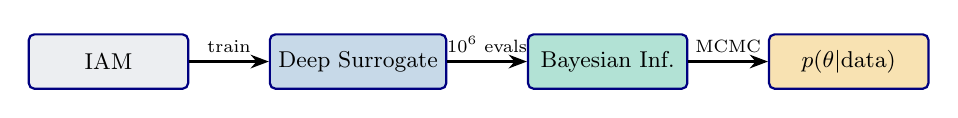
\begin{tikzpicture}[
    mlstep/.style={rectangle, draw=uzhblue, fill=uzhgreylight,
        minimum width=2.2cm, minimum height=0.75cm, font=\small,
        rounded corners=2pt, thick},
    >=Stealth, scale=0.92, transform shape
]
\node[mlstep] (model) {IAM};
\node[mlstep, right=1.1cm of model, fill=softblue!30] (surr) {Deep Surrogate};
\node[mlstep, right=1.1cm of surr, fill=softgreen!30] (bayes) {Bayesian Inf.};
\node[mlstep, right=1.1cm of bayes, fill=softorange!30] (post) {$p(\theta|\text{data})$};

\draw[->, thick] (model) -- node[above, font=\scriptsize]{train} (surr);
\draw[->, thick] (surr) -- node[above, font=\scriptsize]{$10^6$ evals} (bayes);
\draw[->, thick] (bayes) -- node[above, font=\scriptsize]{MCMC} (post);
\end{tikzpicture}
\end{center}

\vspace{0.2cm}
\begin{itemize}\small\itemsep1pt
  \item Surrogate over \emphc{100+ climate and economic parameters}
  \item Posterior distributions of \emphc{damage functions} and \emphc{optimal carbon tax}
  \item MCMC requires millions of model evaluations, only feasible with a surrogate
\end{itemize}
\end{frame}

% --- Slide 12: Application III — Optimal Policy ---
\begin{frame}{Application III: Optimal Policy}
K\"ubler, Scheidegger \& Surbek (2025):

\vspace{0.3cm}
\begin{itemize}
  \item High-dimensional integrated assessment model (IAM)
  \item \emphc{GP surrogate + Bayesian Active Learning (BAL)} for the value function
  \item GP provides \emph{uncertainty quantification} at each point
  \item BAL selects training points where uncertainty is highest
  \item Result: optimal carbon tax policy with \emphc{rigorous error bounds}
\end{itemize}

\vspace{0.3cm}
\begin{alertblock}{Preview}
Parts III and IV of this lecture introduce \emphc{Gaussian Processes} and \emphc{Bayesian Active Learning} --- the tools behind this application.
\end{alertblock}
\end{frame}

% --- Slide 12b: Application IV — Implied Volatility Surface ---
\begin{frame}{Application IV: The Implied Volatility Surface}
\textbf{Goal:} Learn the mapping from option characteristics to implied volatility.
\[
\sigma_{IV} = \phi(K, T, S_0, r, \theta_{\text{model}})
\]

\vspace{0.15cm}
\begin{center}
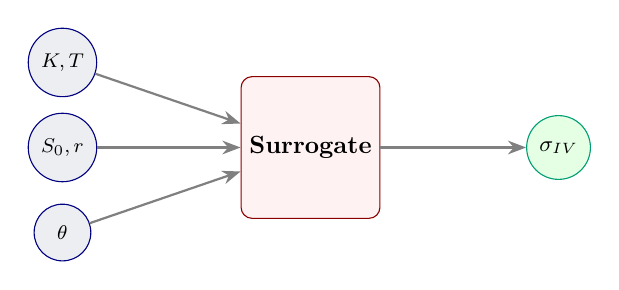
\begin{tikzpicture}[scale=0.9, transform shape,
    node distance=1.8cm,
    input/.style={circle, draw=uzhblue, fill=uzhgreylight, minimum size=0.8cm, font=\footnotesize},
    hidden/.style={rectangle, draw=darkred, fill=red!5, minimum width=1.8cm, minimum height=2cm, rounded corners},
    output/.style={circle, draw=softgreen, fill=green!10, minimum size=0.9cm, font=\small},
    arr/.style={-Stealth, thick, gray}
]
    \node[input] (K) at (0, 1.2) {$K, T$};
    \node[input] (S) at (0, 0) {$S_0, r$};
    \node[input] (P) at (0, -1.2) {$\theta$};
    \node[hidden] (net) at (3.5, 0) {\textbf{Surrogate}};
    \node[output] (IV) at (7, 0) {$\sigma_{IV}$};
    \draw[arr] (K) -- (net);
    \draw[arr] (S) -- (net);
    \draw[arr] (P) -- (net);
    \draw[arr] (net) -- (IV);
\end{tikzpicture}
\end{center}

\vspace{0.15cm}
{\small\textbf{Benefits:}
\begin{itemize}\itemsep0pt
    \item \textbf{Calibration:} Invert the surrogate to find $\theta_{\text{mod}}$ matching market prices.
    \item \textbf{Arbitrage-free:} Can enforce constraints (no calendar/butterfly arb) in the loss.
    \item \textbf{Speed:} Enables real-time pricing for complex stochastic volatility models.
\end{itemize}}
\end{frame}

% --- Slide 13: Pseudo-States — Concrete Use Cases ---
\begin{frame}{Pseudo-States: Concrete Use Cases}
\begin{block}{1. Exploring parameter distributions}
Surrogate $\phi(s, \theta)$ maps \emph{any} parameter $\theta$ to the model output instantly:
\begin{itemize}\setlength{\itemsep}{2pt}
  \item Draw $\theta^{(j)} \sim p(\theta)$ from a prior or posterior distribution
  \item Evaluate $\phi(s, \theta^{(j)})$ for each draw --- \emphc{no re-solving}
  \item Obtain the full distribution of outcomes: $\{y^{(j)}\}_{j=1}^M$
\end{itemize}
$\Rightarrow$ \emphc{Bayesian inference, sensitivity analysis, robust policy design}
\end{block}

\vspace{0.2cm}
\begin{exampleblock}{Example: Climate--economy models}
\begin{itemize}\setlength{\itemsep}{2pt}
  \item Parameters: climate sensitivity, damage curvature, discount rate
  \item Surrogate over 100+ parameters trained once ($\sim$hours)
  \item MCMC posterior with $10^6$ evaluations ($\sim$minutes with surrogate)
\end{itemize}
\end{exampleblock}
\end{frame}

% --- Slide 14: Pseudo-States — Policy Parameterization ---
\begin{frame}{Pseudo-States: Policy Parameterization}
\begin{block}{2. Parameterizing policies}
Include \emphc{policy parameters} $\theta_{\text{pol}}$ as pseudo-states.  Optimize via autograd:
\vspace{-4pt}
\[
\theta_{\text{pol}}^* = \argmax_{\theta_{\text{pol}}} \;\phi\bigl(s,\, \theta_{\text{model}},\, \theta_{\text{pol}}\bigr)
\]
\vspace{-6pt}
\end{block}

\vspace{0.1cm}
\begin{columns}[T]
\begin{column}{0.48\textwidth}
\begin{exampleblock}{Carbon tax}
\begin{itemize}\setlength{\itemsep}{0pt}
  \item Policy: tax trajectory $\theta_{\text{pol}}$
  \item Model: climate sensitivity $\theta_{\text{model}}$
  \item Optimal tax for each $\theta_{\text{model}}$
\end{itemize}
\end{exampleblock}
\end{column}
\begin{column}{0.48\textwidth}
\begin{exampleblock}{Monetary policy}
\begin{itemize}\setlength{\itemsep}{0pt}
  \item Policy: Taylor rule coefficients
  \item Model: preference / technology shocks
  \item Optimal rule via gradient descent
\end{itemize}
\end{exampleblock}
\end{column}
\end{columns}

\vspace{0.15cm}
\emphc{Key:} evaluate welfare for \emph{any} model + policy configuration instantly $\Rightarrow$ no re-solving.
\end{frame}

% --- Slide 15: Sources of Approximation Error ---
\begin{frame}{Sources of Approximation Error}
\begin{center}
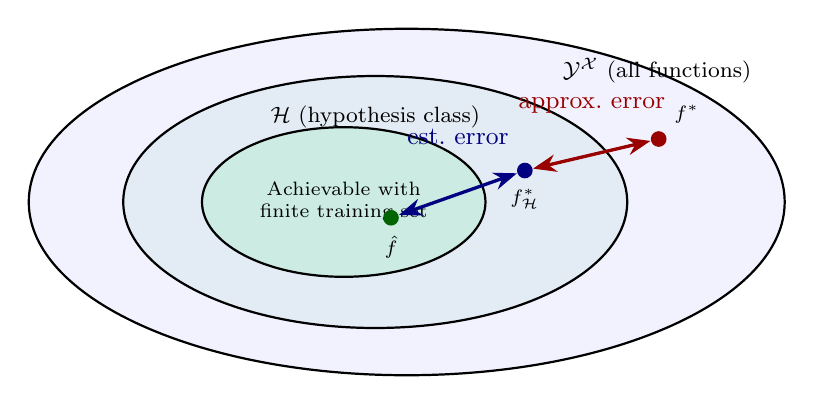
\begin{tikzpicture}[
    every node/.style={font=\footnotesize},
    >=Stealth
]
% Outer set: all functions
\draw[thick, fill=blue!5, rounded corners=8pt]
    (0,0) ellipse (4.8cm and 2.2cm);
\node[anchor=north east] at (4.5,1.95) {$\mathcal{Y}^{\mathcal{X}}$ (all functions)};

% Hypothesis class
\draw[thick, fill=softblue!15, rounded corners=6pt]
    (-0.4,0) ellipse (3.2cm and 1.6cm);
\node[anchor=north] at (-0.4,1.35) {$\mathcal{H}$ (hypothesis class)};

% Achievable with finite data
\draw[thick, fill=softgreen!20, rounded corners=4pt]
    (-0.8,0) ellipse (1.8cm and 0.95cm);
\node[font=\scriptsize, text width=2.5cm, align=center] at (-0.8,0) {Achievable with\\finite training set};

% Target function
\node[circle, fill=harvardcrimson, inner sep=2pt, label={[font=\scriptsize]above right:$f^*$}] (fstar) at (3.2,0.8) {};

% Best in H
\node[circle, fill=uzhblue, inner sep=2pt, label={[font=\scriptsize]below:$f_{\mathcal{H}}^*$}] (fH) at (1.5,0.4) {};

% Trained model
\node[circle, fill=darkgreen, inner sep=2pt, label={[font=\scriptsize]below:$\hat{f}$}] (fhat) at (-0.2,-0.2) {};

% Error arrows with readable labels
\draw[<->, very thick, harvardcrimson] (fstar) -- (fH);
\node[font=\small, text=harvardcrimson, above] at (2.35,1.0) {approx.\ error};
\draw[<->, very thick, uzhblue] (fH) -- (fhat);
\node[font=\small, text=uzhblue, above] at (0.65,0.6) {est.\ error};
\end{tikzpicture}
\end{center}

\vspace{0.1cm}
\begin{itemize}
  \item \textbf{Approximation error:} $f^*$ may not lie in $\mathcal{H}$ $\Rightarrow$ increase network capacity.
  \item \textbf{Estimation error:} finite data $\Rightarrow$ mitigated by generating more training points.
  \item For surrogates, \emphc{estimation error $\to 0$} as we can always generate more data.
\end{itemize}
\end{frame}

% --- Slide 14: Practical Tips ---
\begin{frame}{Practical Tips for Surrogate Training}
\begin{columns}[T]
\begin{column}{0.48\textwidth}
\begin{block}{Architecture}
\begin{itemize}\setlength{\itemsep}{1pt}
  \item Swish activation ($x \cdot \sigma(x)$)
  \item 3--5 hidden layers, 128--512 neurons
  \item Linear output (no activation)
\end{itemize}
\end{block}

\begin{block}{Training}
\begin{itemize}\setlength{\itemsep}{1pt}
  \item $m \geq 10^5$ samples (cheap to generate)
  \item Adam, LR $10^{-3}$, reduce on plateau
  \item Hundreds of epochs (no overfit risk)
\end{itemize}
\end{block}
\end{column}

\begin{column}{0.48\textwidth}
\begin{block}{Validation}
\begin{itemize}\setlength{\itemsep}{1pt}
  \item Held-out test set
  \item Max / mean absolute error, $R^2$
  \item Scatter: prediction vs.\ truth
\end{itemize}
\end{block}

\begin{block}{Loss functions}
\begin{itemize}\setlength{\itemsep}{1pt}
  \item MSE: $\frac{1}{m}\sum_i (\phi_i - y_i)^2$
  \item Relative $L^1$: $\frac{1}{m}\sum_i |(\phi_i - y_i)/y_i|$
\end{itemize}
\end{block}
\end{column}
\end{columns}
\end{frame}

% --- Slide 15: Summary Part I ---
\begin{frame}{Summary: Deep Surrogate Models}
\begin{enumerate}
  \item \textbf{Surrogates} = cheap, accurate replicas of expensive models.
  \item \textbf{Pseudo-states} ($\theta$ as extra inputs) unlock:
  \begin{itemize}
    \item Structural estimation (GMM in seconds)
    \item Uncertainty quantification (MCMC with surrogate)
    \item Optimal policy design
  \end{itemize}
  \item \textbf{Key advantage:} unlimited training data $\Rightarrow$ no overfitting.
  \item \textbf{Speed:} orders of magnitude faster than original model.
\end{enumerate}

\vspace{0.3cm}
\begin{block}{Hands-on}
\textbf{Notebook:} \texttt{01\_Surrogate\_Primer.ipynb} --- Black--Scholes surrogate with implied volatility inversion.
\end{block}
\end{frame}

% ============================================================================
% PART II: GAUSSIAN PROCESS REGRESSION
% ============================================================================
\section{Gaussian Process Regression}

% --- Slide 16: Why Gaussian Processes? ---
\begin{frame}{Why Gaussian Processes?}
\begin{itemize}
  \item \textbf{Nonparametric:} No fixed architecture; the model grows with data.
  \item \textbf{Built-in uncertainty quantification:} Posterior mean \emph{and} variance at every point.
  \item \textbf{Principled kernel selection:} Encode prior beliefs about smoothness, periodicity, etc.
  \item \textbf{Hyperparameter learning:} Marginal likelihood provides a principled objective.
\end{itemize}

\vspace{0.3cm}
\begin{alertblock}{Complementary to DNNs}
\begin{itemize}
  \item GPs: best for moderate dimensions ($d \leq 10$) with built-in UQ.
  \item DNNs: best for high dimensions ($d \gg 10$) with large data.
  \item Combining both is a powerful strategy (cf.\ slide~9).
\end{itemize}
\end{alertblock}

\vspace{0.15cm}
{\tiny \textbf{Foundations:} Rasmussen \& Williams (2006); MacKay (1992); Krause, Singh \& Guestrin (2008).
\textbf{In DP:} Engel, Mannor \& Meir (2005); Deisenroth, Rasmussen \& Peters (2009).
\textbf{Sparse / scalable:} Titsias (2009); Hensman, Fusi \& Lawrence (2013).}
\end{frame}

% --- Foundational slides (from Bundesbank version) ---
\begin{frame}{Recall: Multivariate Gaussians}
\begin{columns}[T]
\begin{column}{0.45\textwidth}
A random vector $\bm{x} \in \R^d$ is \emphc{multivariate Gaussian} if
\[
\bm{x} \sim \mathcal{N}(\bm{\mu}, \Sigma)
\]
with density
{\small
\[
p(\bm{x}) \propto
\exp\!\Bigl(-\tfrac{1}{2}(\bm{x}\!-\!\bm{\mu})^\top \Sigma^{-1}(\bm{x}\!-\!\bm{\mu})\Bigr)
\]
}

\vspace{0.2cm}
\begin{block}{Key fact}
A multivariate Gaussian is \emphc{fully characterized} by its mean vector $\bm{\mu}$ and covariance matrix $\Sigma$.
\end{block}
\end{column}

\begin{column}{0.52\textwidth}
\begin{center}
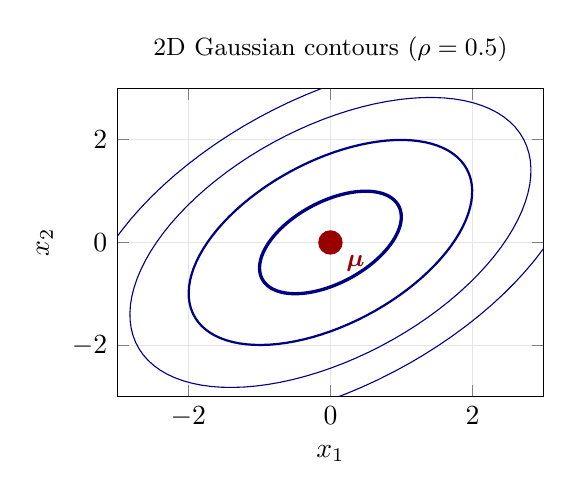
\begin{tikzpicture}
\begin{axis}[
    width=7cm, height=5.5cm,
    xlabel={$x_1$}, ylabel={$x_2$},
    xmin=-3, xmax=3, ymin=-3, ymax=3,
    grid=major, grid style={gray!20},
    every axis plot/.append style={no markers},
    title={\small 2D Gaussian contours ($\rho=0.5$)},
]
\addplot[uzhblue, very thick, domain=0:360, samples=100]
    ({0.707*(1.22*cos(x) - 0.707*sin(x))}, {0.707*(1.22*cos(x) + 0.707*sin(x))});
\addplot[uzhblue, thick, domain=0:360, samples=100]
    ({1.414*(1.22*cos(x) - 0.707*sin(x))}, {1.414*(1.22*cos(x) + 0.707*sin(x))});
\addplot[uzhblue, domain=0:360, samples=100]
    ({2.0*(1.22*cos(x) - 0.707*sin(x))}, {2.0*(1.22*cos(x) + 0.707*sin(x))});
\addplot[uzhblue, thin, domain=0:360, samples=100]
    ({2.5*(1.22*cos(x) - 0.707*sin(x))}, {2.5*(1.22*cos(x) + 0.707*sin(x))});
\addplot[only marks, mark=+, mark size=4pt, harvardcrimson, thick] coordinates {(0,0)};
\node[font=\small, harvardcrimson] at (axis cs:0.35,-0.4) {$\bm{\mu}$};
\end{axis}
\end{tikzpicture}
\end{center}
\end{column}
\end{columns}
\end{frame}

\begin{frame}{Joint and Conditional Distributions}
\begin{columns}[T]
\begin{column}{0.48\textwidth}
\textbf{Joint distribution:}
\[
\begin{pmatrix} x_1 \\ x_2 \end{pmatrix}
\sim \mathcal{N}\!\left(
\begin{pmatrix} \mu_1 \\ \mu_2 \end{pmatrix},
\begin{pmatrix} \Sigma_{11} & \Sigma_{12} \\ \Sigma_{21} & \Sigma_{22} \end{pmatrix}
\right)
\]

\vspace{0.3cm}
\textbf{Conditional distribution:}
\begin{align*}
\mu_{1|2} &= \mu_1 + \Sigma_{12}\Sigma_{22}^{-1}(x_2 - \mu_2)\\
\Sigma_{1|2} &= \Sigma_{11} - \Sigma_{12}\Sigma_{22}^{-1}\Sigma_{21}
\end{align*}

\vspace{0.1cm}
\emphc{This is the mathematical engine behind GP regression.}
\end{column}

\begin{column}{0.50\textwidth}
\begin{center}
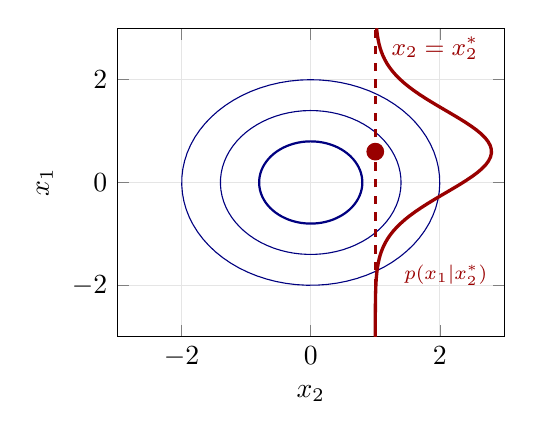
\begin{tikzpicture}
\begin{axis}[
    width=6.5cm, height=5.5cm,
    xlabel={$x_2$}, ylabel={$x_1$},
    xmin=-3, xmax=3, ymin=-3, ymax=3,
    grid=major, grid style={gray!20},
    every axis plot/.append style={no markers},
]
\addplot[uzhblue, thick, domain=0:360, samples=80]
    ({0.8*(0.894*cos(x) - 0.447*sin(x))}, {0.8*(0.447*cos(x) + 0.894*sin(x))});
\addplot[uzhblue, domain=0:360, samples=80]
    ({1.4*(0.894*cos(x) - 0.447*sin(x))}, {1.4*(0.447*cos(x) + 0.894*sin(x))});
\addplot[uzhblue, thin, domain=0:360, samples=80]
    ({2.0*(0.894*cos(x) - 0.447*sin(x))}, {2.0*(0.447*cos(x) + 0.894*sin(x))});
\draw[harvardcrimson, very thick, dashed] (axis cs:1,-3) -- (axis cs:1,3);
\node[font=\small, harvardcrimson, anchor=south west] at (axis cs:1.1,2.2) {$x_2 = x_2^*$};
\addplot[harvardcrimson, very thick, domain=-3:3, samples=80]
    ({1 + 1.8*exp(-(x-0.6)^2/(2*0.64))}, {x});
\node[font=\scriptsize, harvardcrimson, anchor=west, inner sep=1pt]
    at (axis cs:1.4,-1.8) {$p(x_1|x_2^*)$};
\addplot[only marks, mark=*, mark size=3pt, harvardcrimson] coordinates {(1,0.6)};
\end{axis}
\end{tikzpicture}
\end{center}
{\small ``Slicing'' the joint at $x_2 = x_2^*$ yields a 1D Gaussian.}
\end{column}
\end{columns}
\end{frame}

\begin{frame}{From Observations to Interpolation}
\vspace{-0.2cm}
\begin{columns}[T]
\begin{column}{0.38\textwidth}
\begin{center}
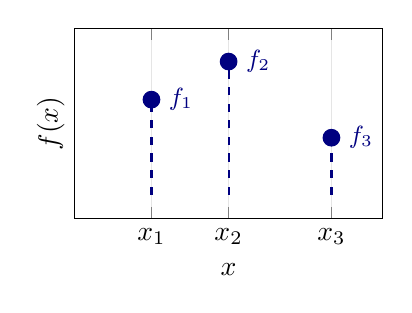
\begin{tikzpicture}
\begin{axis}[
    width=5.5cm, height=4cm,
    xlabel={$x$}, ylabel={$f(x)$},
    xmin=-0.5, xmax=5.5, ymin=-0.5, ymax=3.5,
    grid=major, grid style={gray!20},
    xtick={1,2.5,4.5},
    xticklabels={$x_1$,$x_2$,$x_3$},
    ytick=\empty,
    every axis plot/.append style={no markers},
]
\addplot[uzhblue, thick, dashed] coordinates {(1,0) (1,2.0)};
\addplot[uzhblue, thick, dashed] coordinates {(2.5,0) (2.5,2.8)};
\addplot[uzhblue, thick, dashed] coordinates {(4.5,0) (4.5,1.2)};
\addplot[only marks, mark=*, mark size=3pt, uzhblue] coordinates
    {(1,2.0) (2.5,2.8) (4.5,1.2)};
\node[font=\small, uzhblue, anchor=west] at (axis cs:1.15,2.0) {$f_1$};
\node[font=\small, uzhblue, anchor=west] at (axis cs:2.65,2.8) {$f_2$};
\node[font=\small, uzhblue, anchor=west] at (axis cs:4.65,1.2) {$f_3$};
\end{axis}
\end{tikzpicture}
\end{center}
\end{column}

\begin{column}{0.60\textwidth}
\textbf{Assume} function values are jointly Gaussian:
\vspace{-0.2cm}
{\small
\[
\begin{pmatrix} f_1 \\ f_2 \\ f_3 \end{pmatrix}
\sim \mathcal{N}\!\left(
\bm{0},\;
\begin{pmatrix} K_{11} & K_{12} & K_{13} \\ K_{21} & K_{22} & K_{23} \\ K_{31} & K_{32} & K_{33} \end{pmatrix}
\right)
\]
}

\vspace{-0.1cm}
\emphc{Nearby points ($f_1, f_2$) should be more correlated than distant ones ($f_1, f_3$).}

\vspace{0.1cm}
\textbf{Example:}\;
$K = \bigl(\begin{smallmatrix} 1.0 & 0.7 & 0.2 \\ 0.7 & 1.0 & 0.6 \\ 0.2 & 0.6 & 1.0 \end{smallmatrix}\bigr)$

\vspace{0.15cm}
Covariance via a \emphc{kernel function}: $K_{ij} = k(x_i, x_j)$

\vspace{0.1cm}
{\small $\Rightarrow$ The kernel encodes our prior belief about function smoothness.}
\end{column}
\end{columns}
\end{frame}

% --- GP — A Distribution Over Functions ---
\begin{frame}{GP: A Distribution Over Functions}
\begin{block}{Definition}
A \emphc{Gaussian Process} is a collection of random variables, any finite number of which have a joint Gaussian distribution:
\[
f(\x) \sim \mathcal{GP}\bigl(\mu(\x),\; k(\x, \x')\bigr).
\]
\end{block}

\begin{itemize}
  \item \textbf{Mean function:} $\mu(\x) = \E{f(\x)}$ \quad (often set to $0$).
  \item \textbf{Covariance function (kernel):} $k(\x,\x') = \E{(f(\x)-\mu(\x))(f(\x')-\mu(\x'))^\top}$.
\end{itemize}

\vspace{0.3cm}
\begin{center}
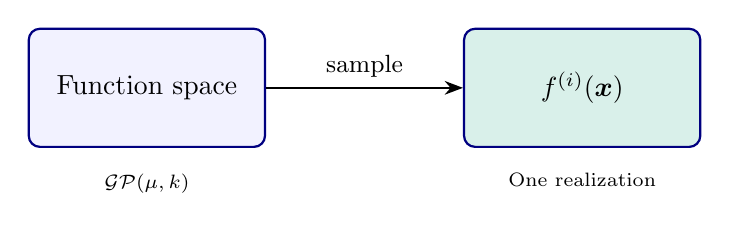
\begin{tikzpicture}[>=Stealth]
\node[draw=uzhblue, thick, rounded corners, fill=blue!5,
      minimum width=3cm, minimum height=1.5cm] (fspace) {Function space};
\node[right=2.5cm of fspace, draw=uzhblue, thick, rounded corners, fill=softgreen!15,
      minimum width=3cm, minimum height=1.5cm] (sample) {$f^{(i)}(\x)$};
\draw[->, thick] (fspace) -- node[above, font=\small]{sample} (sample);
\node[below=0.2cm of fspace, font=\scriptsize] {$\mathcal{GP}(\mu, k)$};
\node[below=0.2cm of sample, font=\scriptsize] {One realization};
\end{tikzpicture}
\end{center}
\end{frame}

% --- Slide 18: The Squared Exponential Kernel ---
\begin{frame}{The Squared Exponential (RBF) Kernel}
\[
k_{SE}(x, x') = \sigma_f^2 \exp\!\left(-\frac{(x - x')^2}{2\ell^2}\right)
\]

\begin{itemize}
  \item $\ell$ = \textbf{length scale} (horizontal correlation range)
  \item $\sigma_f^2$ = \textbf{signal variance} (vertical scale)
\end{itemize}

\vspace{0.2cm}
\begin{center}
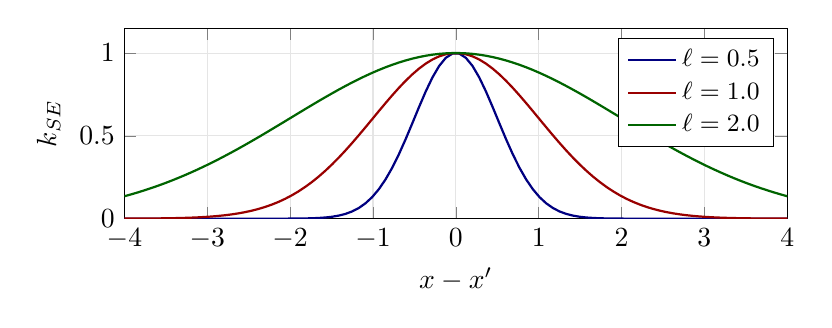
\begin{tikzpicture}
\begin{axis}[
    width=10cm, height=4cm,
    xlabel={$x - x'$}, ylabel={$k_{SE}$},
    xmin=-4, xmax=4, ymin=0, ymax=1.15,
    legend style={at={(0.98,0.95)}, anchor=north east, font=\small},
    grid=major, grid style={gray!20},
    every axis plot/.append style={thick, no markers},
]
\addplot[uzhblue, domain=-4:4, samples=100] {exp(-x^2/(2*0.5^2))};
\addlegendentry{$\ell=0.5$}
\addplot[harvardcrimson, domain=-4:4, samples=100] {exp(-x^2/(2*1.0^2))};
\addlegendentry{$\ell=1.0$}
\addplot[darkgreen, domain=-4:4, samples=100] {exp(-x^2/(2*2.0^2))};
\addlegendentry{$\ell=2.0$}
\end{axis}
\end{tikzpicture}
\end{center}

{\small Larger $\ell$ $\Rightarrow$ smoother functions; smaller $\ell$ $\Rightarrow$ more wiggly.}
\end{frame}

% --- Kernel slides (from Bundesbank version) ---
\begin{frame}{The Mat\'ern Kernel Family}
\vspace{-0.2cm}
{\small
$k_{\text{Mat}}(r) = \sigma^2 \frac{2^{1-\nu}}{\Gamma(\nu)}
\bigl(\frac{\sqrt{2\nu}\,r}{\ell}\bigr)^{\!\nu}
K_\nu\!\bigl(\frac{\sqrt{2\nu}\,r}{\ell}\bigr),
\quad r = |x - x'|$}

\vspace{-0.2cm}
\begin{center}
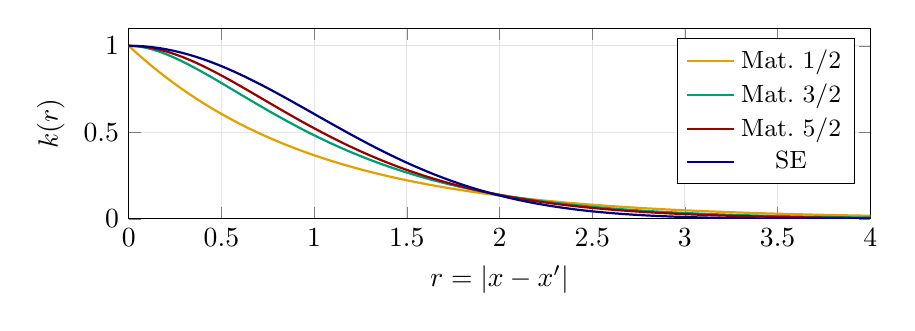
\begin{tikzpicture}
\begin{axis}[
    width=11cm, height=4cm,
    xlabel={$r = |x - x'|$}, ylabel={$k(r)$},
    xmin=0, xmax=4, ymin=0, ymax=1.1,
    grid=major, grid style={gray!20},
    every axis plot/.append style={thick, no markers},
    legend style={at={(0.98,0.95)}, anchor=north east, font=\small},
]
\addplot[softorange, domain=0:4, samples=100] {exp(-x)};
\addlegendentry{Mat.\ 1/2}
\addplot[softgreen, domain=0:4, samples=100] {(1+1.732*x)*exp(-1.732*x)};
\addlegendentry{Mat.\ 3/2}
\addplot[harvardcrimson, domain=0:4, samples=100] {(1+2.236*x+5/3*x^2)*exp(-2.236*x)};
\addlegendentry{Mat.\ 5/2}
\addplot[uzhblue, domain=0:4, samples=100] {exp(-x^2/2)};
\addlegendentry{SE}
\end{axis}
\end{tikzpicture}
\end{center}

\vspace{-0.2cm}
{\small
\begin{itemize}\setlength{\itemsep}{0pt}
  \item $\nu$ controls \emphc{smoothness}: $\nu\!=\!3/2$ $\Rightarrow$ once differentiable;\; $\nu\!=\!5/2$ $\Rightarrow$ twice;\; SE $\Rightarrow$ $\infty$-smooth.
  \item \textbf{Use case:} Mat\'ern when the true function is \emph{not} infinitely smooth (e.g., has kinks).
\end{itemize}}
\end{frame}

\begin{frame}[shrink=5]{Combining Kernels}
Kernels can be \emphc{added} and \emphc{multiplied} to compose complex priors from simple blocks.

\vspace{0.3cm}
\begin{columns}[T]
\column{0.55\textwidth}
\begin{center}
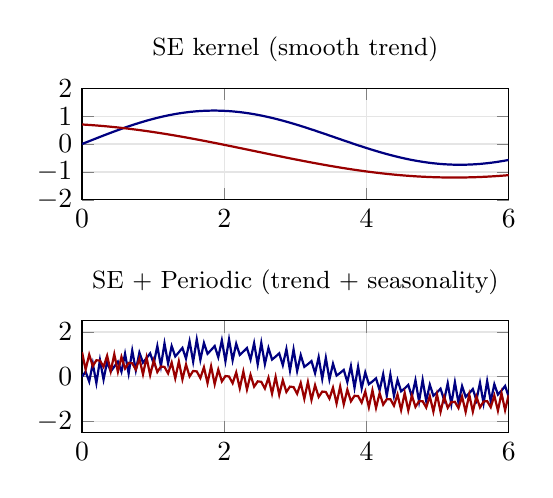
\begin{tikzpicture}
\begin{axis}[
    name=kse,
    width=7cm, height=3cm,
    title={\small SE kernel (smooth trend)},
    xmin=0, xmax=6, ymin=-2, ymax=2,
    grid=major, grid style={gray!20},
    every axis plot/.append style={thick, no markers},
]
\addplot[uzhblue, domain=0:6, samples=80] {sin(deg(0.9*x)) + 0.3*sin(deg(0.4*x))};
\addplot[harvardcrimson, domain=0:6, samples=80] {0.7*cos(deg(0.6*x)) - 0.5*sin(deg(0.3*x))};
\end{axis}

\begin{axis}[
    at={(kse.below south)}, anchor=above north, yshift=-0.3cm,
    width=7cm, height=3cm,
    title={\small SE $+$ Periodic (trend + seasonality)},
    xmin=0, xmax=6, ymin=-2.5, ymax=2.5,
    grid=major, grid style={gray!20},
    every axis plot/.append style={thick, no markers},
]
\addplot[uzhblue, domain=0:6, samples=120]
    {sin(deg(0.9*x)) + 0.3*sin(deg(0.4*x)) + 0.5*sin(deg(180*x))};
\addplot[harvardcrimson, domain=0:6, samples=120]
    {0.7*cos(deg(0.6*x)) - 0.5*sin(deg(0.3*x)) + 0.4*cos(deg(180*x))};
\end{axis}
\end{tikzpicture}
\end{center}

\column{0.42\textwidth}
\begin{block}{Kernel algebra}
\begin{itemize}\setlength{\itemsep}{3pt}
  \item \textbf{$k_1 + k_2$} (OR):\\
  high if \emph{either} is high\\
  $\Rightarrow$ trend + seasonality
  \item \textbf{$k_1 \times k_2$} (AND):\\
  high only if \emph{both} high\\
  $\Rightarrow$ locally periodic
\end{itemize}
\end{block}

\vspace{0.3cm}
{\small \emphc{Compose complex priors} from simple building blocks.}
\end{columns}
\end{frame}

% --- Sampling from the GP Prior ---
\begin{frame}{Sampling from the GP Prior}
\begin{columns}[T]
\begin{column}{0.42\textwidth}
\begin{block}{Algorithm}
\begin{enumerate}\setlength{\itemsep}{1pt}
  \item Grid $x_{1:N}$ over domain
  \item $K_{ij} = k(x_i, x_j)$
  \item Cholesky: $K = LL^\top$
  \item $\bm{f}^{(s)} = L \cdot \bm{u}$, $\bm{u} \sim \mathcal{N}(\bm{0}, I)$
\end{enumerate}
\end{block}
\vspace{0.2cm}
{\small Five functions drawn from a GP prior with SE kernel ($\ell=1$, $\sigma_f=1$).}
\end{column}
\begin{column}{0.56\textwidth}
\begin{center}
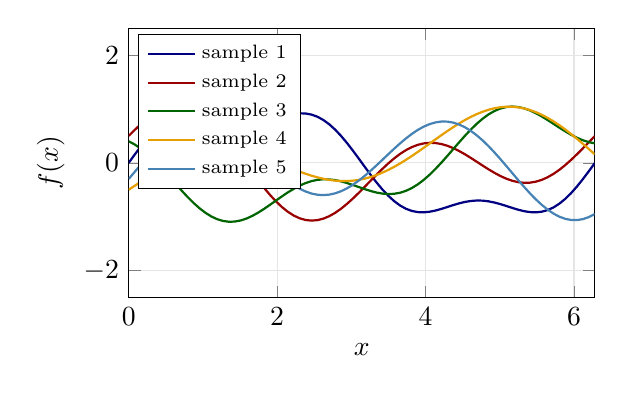
\begin{tikzpicture}
\begin{axis}[
    width=7.5cm, height=5cm,
    xlabel={$x$}, ylabel={$f(x)$},
    xmin=0, xmax=6.28, ymin=-2.5, ymax=2.5,
    grid=major, grid style={gray!20},
    every axis plot/.append style={thick, no markers},
    legend style={at={(0.02,0.98)}, anchor=north west, font=\scriptsize},
]
\addplot[uzhblue, domain=0:6.28, samples=80] {sin(deg(x)) + 0.3*sin(deg(3*x))};
\addlegendentry{sample 1}
\addplot[harvardcrimson, domain=0:6.28, samples=80] {0.5*cos(deg(x)) + 0.7*sin(deg(2*x))};
\addlegendentry{sample 2}
\addplot[darkgreen, domain=0:6.28, samples=80] {-0.8*sin(deg(0.8*x)) + 0.4*cos(deg(2.5*x))};
\addlegendentry{sample 3}
\addplot[softorange, domain=0:6.28, samples=80] {0.6*sin(deg(1.5*x)) - 0.5*cos(deg(0.7*x))};
\addlegendentry{sample 4}
\addplot[softblue, domain=0:6.28, samples=80] {-0.3*cos(deg(1.2*x)) + 0.9*sin(deg(1.8*x))};
\addlegendentry{sample 5}
\end{axis}
\end{tikzpicture}
\end{center}
\end{column}
\end{columns}
\end{frame}

% --- Slide 20: From Prior to Posterior ---
\begin{frame}{From Prior to Posterior: Bayes Rule}
\begin{itemize}
  \item \textbf{Training set:} $\mathcal{D} = \{(\x_i, y_i)\}_{i=1}^n$.
  \item \textbf{Test points:} $\X_*$ where we want predictions.
  \item Joint distribution of training outputs $\bm{f}$ and test outputs $\bm{f}_*$ is Gaussian.
\end{itemize}

\vspace{0.3cm}
\begin{center}
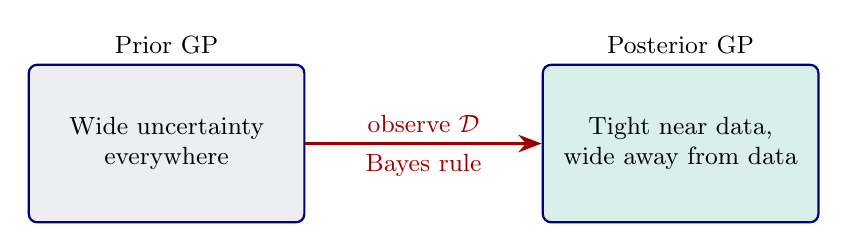
\begin{tikzpicture}[
    mlstep/.style={rectangle, draw=uzhblue, fill=uzhgreylight,
        minimum width=3.5cm, minimum height=2cm, rounded corners=3pt, thick},
    >=Stealth
]
\node[mlstep, label={[font=\small]above:Prior GP}] (prior) {
    \begin{minipage}{3cm}\centering
    \small Wide uncertainty\\everywhere
    \end{minipage}};
\node[mlstep, right=3cm of prior, fill=softgreen!15,
      label={[font=\small]above:Posterior GP}] (post) {
    \begin{minipage}{3cm}\centering
    \small Tight near data,\\wide away from data
    \end{minipage}};
\draw[->, very thick, harvardcrimson] (prior) -- node[above, font=\small]{observe $\mathcal{D}$}
    node[below, font=\small]{\emphc{Bayes rule}} (post);
\end{tikzpicture}
\end{center}

\vspace{0.2cm}
The posterior is \emph{still a GP} --- fully characterized by updated mean and covariance.
\end{frame}

% --- Slide 21: Noiseless GP Regression ---
\begin{frame}{Noiseless GP Regression}
\textbf{Joint distribution:}
\[
\begin{pmatrix} \bm{f} \\ \bm{f}_* \end{pmatrix}
\sim \mathcal{N}\!\left(
\begin{pmatrix} \bm{\mu} \\ \bm{\mu}_* \end{pmatrix},
\begin{pmatrix} K & K_* \\ K_*^\top & K_{**} \end{pmatrix}
\right)
\]

where $K_{ij} = k(\x_i, \x_j)$, \; $(K_*)_{ij} = k(\x_i, \x_*^{(j)})$, \; $(K_{**})_{ij} = k(\x_*^{(i)}, \x_*^{(j)})$.

\vspace{0.3cm}
\textbf{Posterior} (conditioning on $\bm{f}$):
\begin{align}
\bm{\mu}_{*|\mathcal{D}} &= K_*^\top K^{-1}(\bm{f} - \bm{\mu}) + \bm{\mu}_* \label{eq:gp_mean}\\
\Sigma_{*|\mathcal{D}} &= K_{**} - K_*^\top K^{-1} K_* \label{eq:gp_var}
\end{align}

\vspace{0.2cm}
\begin{alertblock}{Key insight}
\begin{itemize}
  \item Near observed data: $K_*^\top K^{-1} K_* \approx K_{**}$ $\Rightarrow$ \emphc{small variance}.
  \item Far from data: $K_*^\top K^{-1} K_* \approx 0$ $\Rightarrow$ \emphc{large variance} (reverts to prior).
\end{itemize}
\end{alertblock}
\end{frame}

% --- Slide 22: Prediction at a Single Test Point ---
\begin{frame}{Prediction at a Single Test Point}
\small
\textbf{Noiseless setting} ($\sigma_y^2 \to 0$ limit; GP interpolates training data). For a single test input $\x_*$:
\vspace{-4pt}
\begin{align}
\bar{f}_* &= \bm{k}_*^\top K^{-1} \bm{f} = \sum_{i=1}^{N} \alpha_i \, k(\x_i, \x_*) \\
\sigma_*^2 &= k(\x_*, \x_*) - \bm{k}_*^\top K^{-1} \bm{k}_*
\end{align}
\vspace{-12pt}

where $\bm{\alpha} = K^{-1}\bm{f}$, $\bm{k}_* = (k(\x_1, \x_*), \dots, k(\x_N, \x_*))^\top$. Noisy form ($K \to K + \sigma_y^2 I$) on next slide.

\begin{block}{Interpretation}
Posterior mean is a \emphc{weighted sum of kernel basis functions} centered at training points:
\vspace{-4pt}
\[
\bar{f}_* = \sum_{i=1}^N \alpha_i \, k(\x_i, \x_*)
\]
\vspace{-10pt}

Each observation $\x_i$ ``pulls'' the prediction via its kernel similarity to $\x_*$.
\end{block}
\end{frame}

% --- Slide 23: GPR with Noisy Data ---
\begin{frame}{GP Regression with Noisy Observations}
\textbf{Observation model:}
\[
y = f(\x) + \varepsilon, \qquad \varepsilon \sim \mathcal{N}(0, \sigma_y^2)
\]

\vspace{0.2cm}
The covariance of \emph{observations} becomes:
\[
\text{cov}[y_p, y_q] = k(\x_p, \x_q) + \sigma_y^2 \delta_{pq}
\]

\vspace{0.2cm}
In matrix form: replace $K$ with
\[
K_y = K + \sigma_y^2 I
\]

\vspace{0.3cm}
\begin{block}{Effect of noise}
\begin{itemize}
  \item Predictions no longer interpolate the data exactly.
  \item Even at training points, there is \emphc{residual uncertainty}.
  \item The noise term $\sigma_y^2 I$ also acts as \emphc{numerical regularization} (``nugget'' / ``jitter'').
\end{itemize}
\end{block}
\end{frame}

% --- Slide 24: Noisy GPR Posterior ---
\begin{frame}{Noisy GPR: Posterior Equations}
\textbf{Posterior mean and variance with noise:}
\begin{align}
\bar{f}_* &= \bm{k}_*^\top (K + \sigma_y^2 I)^{-1} \bm{y} \\
\sigma_*^2 &= k(\x_*, \x_*) - \bm{k}_*^\top (K + \sigma_y^2 I)^{-1} \bm{k}_*
\end{align}

\vspace{0.3cm}
\begin{columns}[T]
\begin{column}{0.48\textwidth}
\textbf{Noiseless} ($\sigma_y^2 = 0$):
\begin{itemize}
  \item Interpolates training points exactly
  \item Variance = 0 at training inputs
  \item Requires $K$ to be positive definite
\end{itemize}
\end{column}
\begin{column}{0.48\textwidth}
\textbf{Noisy} ($\sigma_y^2 > 0$):
\begin{itemize}
  \item Smooths through training points
  \item Variance $> 0$ everywhere
  \item Better numerical conditioning
\end{itemize}
\end{column}
\end{columns}

\vspace{0.3cm}
{\small \textbf{In practice:} Even for noiseless surrogates, adding a small jitter $\sigma_y^2 \sim 10^{-6}$ improves numerical stability.}
\end{frame}

% --- Slide 25: Effect of Kernel Parameters ---
\begin{frame}{The Effect of Kernel Parameters}
\begin{center}
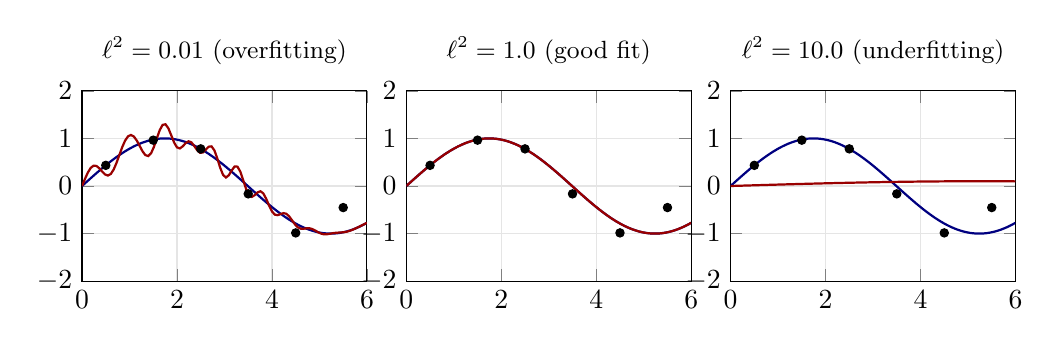
\begin{tikzpicture}
% Panel 1: small length scale (overfit)
\begin{axis}[
    name=plot1,
    width=5.2cm, height=4cm,
    title={\small $\ell^2 = 0.01$ (overfitting)},
    xmin=0, xmax=6, ymin=-2, ymax=2,
    grid=major, grid style={gray!20},
    every axis plot/.append style={no markers},
]
\addplot[uzhblue, thick, domain=0:6, samples=100] {sin(deg(0.9*x))};
\addplot[harvardcrimson, thick, domain=0:6, samples=100]
    {sin(deg(0.9*x)) + 0.3*sin(deg(8*x))*exp(-0.5*(x-1)^2) + 0.2*sin(deg(12*x))*exp(-0.5*(x-3)^2)};
\addplot[only marks, mark=*, mark size=1.5pt] coordinates
    {(0.5,0.434) (1.5,0.963) (2.5,0.780) (3.5,-0.165) (4.5,-0.985) (5.5,-0.453)};
\end{axis}

% Panel 2: good length scale
\begin{axis}[
    name=plot2, at={(plot1.east)}, anchor=west, xshift=0.5cm,
    width=5.2cm, height=4cm,
    title={\small $\ell^2 = 1.0$ (good fit)},
    xmin=0, xmax=6, ymin=-2, ymax=2,
    grid=major, grid style={gray!20},
    every axis plot/.append style={no markers},
]
\addplot[uzhblue, thick, domain=0:6, samples=100] {sin(deg(0.9*x))};
\addplot[harvardcrimson, thick, domain=0:6, samples=100] {sin(deg(0.9*x))};
\addplot[only marks, mark=*, mark size=1.5pt] coordinates
    {(0.5,0.434) (1.5,0.963) (2.5,0.780) (3.5,-0.165) (4.5,-0.985) (5.5,-0.453)};
\end{axis}

% Panel 3: large length scale (underfit)
\begin{axis}[
    name=plot3, at={(plot2.east)}, anchor=west, xshift=0.5cm,
    width=5.2cm, height=4cm,
    title={\small $\ell^2 = 10.0$ (underfitting)},
    xmin=0, xmax=6, ymin=-2, ymax=2,
    grid=major, grid style={gray!20},
    every axis plot/.append style={no markers},
]
\addplot[uzhblue, thick, domain=0:6, samples=100] {sin(deg(0.9*x))};
\addplot[harvardcrimson, thick, domain=0:6, samples=100] {0.1*sin(deg(0.3*x))};
\addplot[only marks, mark=*, mark size=1.5pt] coordinates
    {(0.5,0.434) (1.5,0.963) (2.5,0.780) (3.5,-0.165) (4.5,-0.985) (5.5,-0.453)};
\end{axis}
\end{tikzpicture}
\end{center}

\vspace{0.2cm}
\begin{itemize}
  \item \textcolor{uzhblue}{\textbf{Blue:}} true function $f(x) = \sin(0.9x)$.
  \item \textcolor{harvardcrimson}{\textbf{Red:}} GP posterior mean.
  \item \textbf{Too small $\ell$:} overfits noise/wiggles. \quad \textbf{Too large $\ell$:} underfits, misses structure.
\end{itemize}

$\Rightarrow$ We need a principled way to learn $\ell$ and $\sigma_f^2$.
\end{frame}

% --- Slide 26: Learning Hyperparameters ---
\begin{frame}{Learning Kernel Hyperparameters}
\textbf{Problem:} How to choose $\ell$, $\sigma_f$, $\sigma_y$?  $\Rightarrow$ Maximize the \emphc{marginal likelihood}.

\vspace{0.2cm}
\begin{block}{Marginal likelihood (model evidence)}
\[
\log p(\bm{y}\,|\,\X) = \underbrace{-\tfrac{1}{2}\bm{y}^\top K_y^{-1}\bm{y}}_{\text{data fit}}
\underbrace{-\tfrac{1}{2}\log|K_y|}_{\text{complexity penalty}}
\underbrace{-\tfrac{N}{2}\log(2\pi)}_{\text{constant}}
\]
\end{block}

\vspace{0.1cm}
\begin{columns}[T]
\begin{column}{0.48\textwidth}
\textbf{Intuition:}
\begin{itemize}\setlength{\itemsep}{2pt}
  \item \textbf{Data fit} $\uparrow$: reward explaining observations
  \item \textbf{Complexity} $\downarrow$: penalize overly flexible models
  \item Balance $=$ \emphc{automatic Occam's razor}
\end{itemize}
\end{column}
\begin{column}{0.48\textwidth}
\textbf{Optimization:}
\begin{itemize}\setlength{\itemsep}{2pt}
  \item Gradient ascent on $\log p(\bm{y}|\X)$
  \item Hyperparameters: $\theta = \{\ell, \sigma_f, \sigma_y\}$
  \item Closed-form gradients available
  \item Implemented in scikit-learn, GPyTorch
\end{itemize}
\end{column}
\end{columns}
\end{frame}

% --- New slide: Leave-one-out predictive error ---
\begin{frame}{Leave-One-Out Predictive Error}
\textbf{Idea.} Quantify out-of-sample predictive accuracy without holding out data.

\smallskip
For a GP with training set $\{(\x_i, y_i)\}_{i=1}^n$ and noise variance $\sigma_y^2$:
\begin{equation*}
\mu_{-i}(\x_i) - y_i \;=\; -\frac{[K_y^{-1}\bm y]_i}{[K_y^{-1}]_{ii}}, \qquad
\sigma_{-i}^2(\x_i) \;=\; \frac{1}{[K_y^{-1}]_{ii}}.
\end{equation*}

\smallskip
\textbf{Why it's free.}
\begin{itemize}\itemsep0pt
  \item $K_y^{-1}$ is recovered from the same Cholesky factor used for posterior inference
  \item LOO across all $n$ points: $\mathcal{O}(n^2)$ on top of the existing $\mathcal{O}(n^3)$
  \item No new training, no held-out split lost
\end{itemize}

\smallskip
\textbf{Use cases.} Surrogate-health diagnostic across iterations of GP-VFI (Part IV) and across active-learning rounds in SMM (companion exercise deck).

\medskip
{\scriptsize Closed form: Rasmussen \& Williams (2006), \S5.4.2.}
\end{frame}

% --- Slide 27: GPR Example Code ---
\begin{frame}[fragile]{GPR: Numpy Implementation Sketch}
\begin{lstlisting}[basicstyle=\footnotesize\ttfamily]
import numpy as np
from scipy.linalg import cho_factor, cho_solve

def kernel(X1, X2, l=1.0, sf=1.0):
    sq = np.sum(X1**2,1).reshape(-1,1) \
         + np.sum(X2**2,1) - 2*X1@X2.T
    return sf**2 * np.exp(-0.5 * sq / l**2)

K = kernel(X_tr, X_tr) + 1e-8*np.eye(N)
L, low = cho_factor(K, lower=True)  # Cholesky
alpha = cho_solve((L, low), y_tr)   # weights

Ks = kernel(X_tr, X_te)
mu  = Ks.T @ alpha                  # mean
v   = cho_solve((L, low), Ks)
var = kernel(X_te, X_te) - Ks.T @ v # variance
\end{lstlisting}

\vspace{0.2cm}
{\small See \textbf{Algorithm 2.1} in Rasmussen \& Williams (2006), and notebook \texttt{02\_GP\_and\_BAL.ipynb}.}
\end{frame}

% --- Slide 28: GP in Practice ---
\begin{frame}{GP in Practice: scikit-learn \& GPyTorch}
\begin{columns}[T]
\begin{column}{0.48\textwidth}
\textbf{scikit-learn:}
\begin{itemize}
  \item \texttt{GaussianProcessRegressor}
  \item Automatic hyperparameter tuning via marginal likelihood
  \item Great for prototyping ($N \leq 10^4$)
  \item CPU only
\end{itemize}
\end{column}
\begin{column}{0.48\textwidth}
\textbf{GPyTorch:}
\begin{itemize}
  \item GPU-accelerated GP inference
  \item Scalable to $N > 10^5$ (inducing points, KISS-GP)
  \item Integrates with PyTorch ecosystem
  \item Production-ready
\end{itemize}
\end{column}
\end{columns}

\vspace{0.5cm}
\begin{block}{Hands-on}
\textbf{Notebook:} \texttt{02\_GP\_and\_BAL.ipynb} --- GP regression from scratch, scikit-learn, and Bayesian Active Learning.
\end{block}
\end{frame}

% --- Slide 29: Prediction and Confidence Intervals ---
\begin{frame}[shrink=5]{Prediction \& Confidence Intervals}
\begin{center}
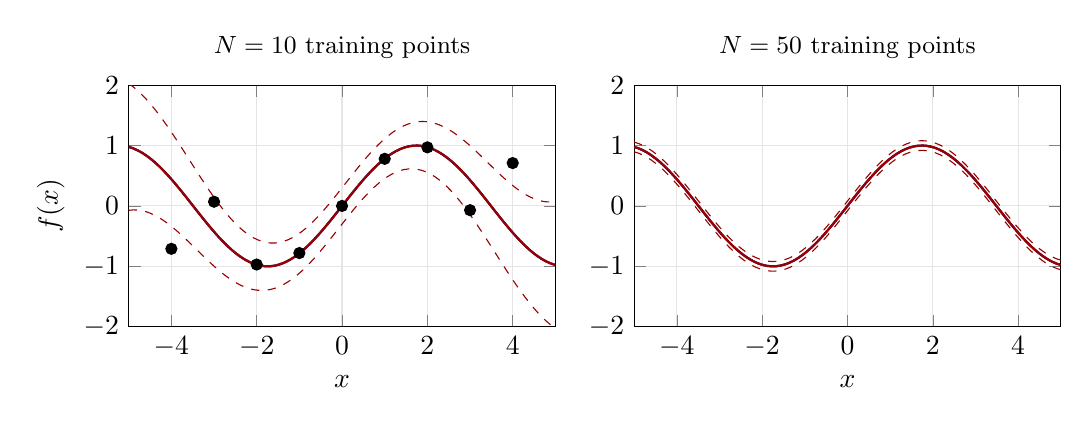
\begin{tikzpicture}
% Left panel: 10 points
\begin{axis}[
    name=left,
    width=7cm, height=4.65cm,
    title={\small $N = 10$ training points},
    xlabel={$x$}, ylabel={$f(x)$},
    xmin=-5, xmax=5, ymin=-2, ymax=2,
    grid=major, grid style={gray!20},
    every axis plot/.append style={no markers},
]
% True function
\addplot[uzhblue, thick, domain=-5:5, samples=100] {sin(deg(0.9*x))/1.0};
% Mean (same as true for good GP)
\addplot[harvardcrimson, thick, domain=-5:5, samples=100] {sin(deg(0.9*x))/1.0};
% CI upper
\addplot[harvardcrimson, thin, dashed, domain=-5:5, samples=100]
    {sin(deg(0.9*x))/1.0 + 0.3*(1 + 0.1*x^2)};
% CI lower
\addplot[harvardcrimson, thin, dashed, domain=-5:5, samples=100]
    {sin(deg(0.9*x))/1.0 - 0.3*(1 + 0.1*x^2)};
% Training points
\addplot[only marks, mark=*, mark size=2pt, black] coordinates
    {(-4,-0.71) (-3,0.07) (-2,-0.97) (-1,-0.78) (0,0)
     (1,0.78) (2,0.97) (3,-0.07) (4,0.71)};
\end{axis}

% Right panel: 50 points
\begin{axis}[
    at={(left.east)}, anchor=west, xshift=1cm,
    width=7cm, height=4.65cm,
    title={\small $N = 50$ training points},
    xlabel={$x$},
    xmin=-5, xmax=5, ymin=-2, ymax=2,
    grid=major, grid style={gray!20},
    every axis plot/.append style={no markers},
]
\addplot[uzhblue, thick, domain=-5:5, samples=100] {sin(deg(0.9*x))/1.0};
\addplot[harvardcrimson, thick, domain=-5:5, samples=100] {sin(deg(0.9*x))/1.0};
\addplot[harvardcrimson, thin, dashed, domain=-5:5, samples=100]
    {sin(deg(0.9*x))/1.0 + 0.08};
\addplot[harvardcrimson, thin, dashed, domain=-5:5, samples=100]
    {sin(deg(0.9*x))/1.0 - 0.08};
\end{axis}
\end{tikzpicture}
\end{center}

\vspace{0.05cm}
{\footnotesize \textcolor{uzhblue}{\textbf{Blue:}} true function. \textcolor{harvardcrimson}{\textbf{Red:}} posterior mean. \textcolor{harvardcrimson}{\textbf{Dashed:}} 95\% confidence interval. \\
More data $\Rightarrow$ tighter confidence intervals.}
\end{frame}

% --- Slide 30: Algorithmic Complexity ---
\begin{frame}[shrink=5]{Algorithmic Complexity}
\begin{block}{Cost of GP inference}
\begin{itemize}
  \item \textbf{Training:} Cholesky decomposition of $K_y \in \R^{N \times N}$: \emphc{$O(N^3)$}.
  \item \textbf{Prediction (per test point):} $O(N)$ for mean, $O(N^2)$ for variance.
  \item \textbf{Hyperparameter optimization:} $O(N^3)$ per gradient step.
\end{itemize}
\end{block}

\vspace{0.15cm}
\begin{block}{Scaling strategies for large $N$}
\begin{itemize}
  \item \textbf{Sparse GPs:} Inducing point methods --- approximate $K$ with rank-$M$ matrix ($M \ll N$), cost $O(NM^2)$.
  \item \textbf{Random features:} Approximate kernel with random Fourier features.
  \item \textbf{GPyTorch:} KISS-GP, structured kernel interpolation, GPU acceleration.
\end{itemize}
\end{block}

\vspace{0.1cm}
{\footnotesize For the surrogate problems in this course ($N \leq 10^4$, $d \leq 10$), standard GPs are sufficient.}
\end{frame}

% --- Slide 31: GPs vs DNNs ---
\begin{frame}{GPs vs DNNs: When to Use Which}
\begin{center}
\footnotesize
\setlength{\tabcolsep}{4pt}
\begin{tabular}{l l l}
\toprule
\textbf{Criterion} & \textbf{Gaussian Processes} & \textbf{Deep Neural Networks} \\
\midrule
Uncertainty quantification & \textcolor{darkgreen}{Built-in (posterior variance)} & \textcolor{darkred}{Requires ensembles / MC dropout} \\
Hyperparameter tuning & \textcolor{darkgreen}{Marginal likelihood} & \textcolor{softorange}{Grid search / Bayesian opt.} \\
Scaling with $N$ & \textcolor{darkred}{$O(N^3)$, limit $\sim 10^4$} & \textcolor{darkgreen}{$O(N)$ per epoch} \\
Scaling with $d$ & \textcolor{darkred}{Curse of dimensionality} & \textcolor{darkgreen}{Handles $d \gg 100$} \\
Small data ($N < 100$) & \textcolor{darkgreen}{Excellent} & \textcolor{darkred}{Typically underfits} \\
Training & \textcolor{darkgreen}{Closed-form} & \textcolor{softorange}{SGD, many epochs} \\
Interpretability & \textcolor{darkgreen}{Kernel encodes prior} & \textcolor{darkred}{Black box} \\
\bottomrule
\end{tabular}
\end{center}

\vspace{0.3cm}
\begin{alertblock}{Rule of thumb}
{\small
\begin{itemize}\itemsep0pt
  \item \textbf{$d \leq 10$, need UQ:} GPs (+ BAL).
  \item \textbf{$d > 10$, large data:} DNNs.
\end{itemize}}
\end{alertblock}
\end{frame}

% --- Slide 31b: Deep Kernel Learning ---
\begin{frame}{Deep Kernel Learning: Neural Features + GP Uncertainty}
\small
\begin{columns}[T]
\begin{column}{0.54\textwidth}
\textbf{Idea:} learn a feature map $\phi_{\theta}(\x)$ with a neural network, then use
\[
\textstyle k_{\text{DKL}}(\x,\x') = k_{\text{base}}\bigl(\phi_{\theta}(\x), \phi_{\theta}(\x')\bigr)
\]
so the GP operates in the learned feature space.

\vspace{0.05cm}
\begin{itemize}\itemsep0.1em
  \item \textbf{Front end:} the DNN learns a geometry where the target is smoother.
  \item \textbf{Back end:} the GP still provides posterior mean and variance.
  \item \textbf{Training:} optimize the feature map and kernel hyperparameters via the GP marginal likelihood.
\end{itemize}

\end{column}

\begin{column}{0.42\textwidth}
\begin{center}
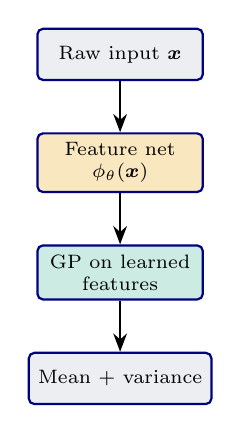
\begin{tikzpicture}[
    box/.style={rectangle, draw=uzhblue, fill=uzhgreylight, rounded corners=2pt,
        minimum width=2.1cm, minimum height=0.65cm, align=center, font=\scriptsize, thick},
    >=Stealth
]
\node[box] (raw) {Raw input $\x$};
\node[box, below=0.65cm of raw, fill=softorange!25] (net) {Feature net\\$\phi_{\theta}(\x)$};
\node[box, below=0.65cm of net, fill=softgreen!20] (gp) {GP on learned\\features};
\node[box, below=0.65cm of gp] (out) {Mean + variance};
\draw[->, thick] (raw) -- (net);
\draw[->, thick] (net) -- (gp);
\draw[->, thick] (gp) -- (out);
\end{tikzpicture}
\end{center}
\end{column}
\end{columns}
\end{frame}

% --- Slide 31c: When DKL Helps ---
\begin{frame}{When Do Deep Kernels Help?}
\begin{columns}[T]
\begin{column}{0.52\textwidth}
\textbf{Standard GP assumption:} Euclidean distance in the \emph{raw input space} is informative.

\vspace{0.2cm}
\textbf{Failure modes:}
\begin{itemize}
  \item Hidden regimes / thresholds / nonstationarity
  \item Inputs are badly warped coordinates of a simple latent state
  \item Moderate-to-high-dimensional raw features with strong correlations
  \item You still need \emphc{uncertainty quantification} or BAL
\end{itemize}
\end{column}

\begin{column}{0.43\textwidth}
\begin{alertblock}{Rule of thumb}
\begin{itemize}
  \item If the input is already low-dimensional and smooth: \textbf{plain GP} is usually enough.
  \item If the latent structure is smooth but the raw geometry is poor: \textbf{DKL} is often the right bridge.
  \item If $d$ is huge and UQ is not central: \textbf{pure DNN surrogate}.
\end{itemize}
\end{alertblock}
\end{column}
\end{columns}

\vspace{0.2cm}
{\small In short: \emphc{DKL answers the question ``Can we combine DNN feature learning with GP uncertainty?''}}
\end{frame}

% --- Slide 32: Summary Part II ---
\begin{frame}{Summary: Gaussian Process Regression}
\begin{enumerate}
  \item \textbf{GPs} = nonparametric Bayesian regression with \emphc{built-in UQ}.
  \item \textbf{Kernel} encodes prior beliefs (smoothness, scale, periodicity).
  \item \textbf{Posterior:} closed-form mean and variance, conditioned on data.
  \item \textbf{Hyperparameters:} learned by maximizing the marginal likelihood (automatic Occam's razor).
  \item \textbf{Limitation:} $O(N^3)$ scaling; best for moderate $N$ and $d$.
  \item \textbf{DKL:} neural feature extractor + GP head = useful when raw inputs are warped or moderately high-dimensional, but you still want UQ.
\end{enumerate}

\vspace{0.3cm}
\textbf{Next:} Use the GP's uncertainty to \emphc{intelligently select training points} --- Bayesian Active Learning.
\end{frame}

% ============================================================================
% PART III: BAYESIAN ACTIVE LEARNING
% ============================================================================
\section{Bayesian Active Learning}

% --- Slide 33: Motivation ---
\begin{frame}{Motivation: Where to Sample?}
\begin{columns}[T]
\begin{column}{0.48\textwidth}
\textbf{Uniform sampling:}
\begin{itemize}
  \item Places points evenly across the domain
  \item Wastes evaluations in smooth regions
  \item Cannot adapt to function complexity
\end{itemize}
\end{column}
\begin{column}{0.48\textwidth}
\textbf{Adaptive / active sampling:}
\begin{itemize}
  \item Concentrates points where the function is \emphc{hard to approximate}
  \item Uses the model's \emphc{uncertainty} to guide selection
  \item Fewer evaluations for the same accuracy
\end{itemize}
\end{column}
\end{columns}

\vspace{0.5cm}
\begin{alertblock}{Key question}
Given a budget of $N$ model evaluations, which input points $\{x_1, \dots, x_N\}$ minimize the overall approximation error?
\end{alertblock}
\end{frame}

% --- Slide 34: BAL — The Idea ---
\begin{frame}{Bayesian Active Learning: The Idea}
\textbf{Use the GP posterior variance to guide sampling.}

\vspace{0.2cm}
\begin{block}{Acquisition / score function}
\vspace{-4pt}
\[
U(\x) = w_{\mathrm{exp}} \cdot \mu(\x) + \frac{w_{\mathrm{var}}}{2}\log\sigma^2(\x)
\]
\vspace{-8pt}
\begin{itemize}\setlength{\itemsep}{1pt}
  \item $\mu(\x)$: posterior mean (\emphc{exploitation} --- sample where function is large)
  \item $\sigma^2(\x)$: posterior variance (\emphc{exploration} --- sample where uncertainty is high)
  \item $w_{\mathrm{exp}}, w_{\mathrm{var}} \geq 0$: trade-off weights (distinct from the AR(1) coefficient $\rho$ and the discount factor $\beta$ used elsewhere).
\end{itemize}
\end{block}

\vspace{0.2cm}
\textbf{Pure exploration} ($w_{\mathrm{exp}} = 0$): maximize $\sigma^2(\x)$, i.e., uncertainty sampling.\\[3pt]
\textbf{Mixed} ($w_{\mathrm{exp}} > 0, w_{\mathrm{var}} > 0$): balance exploration and exploitation.\\[3pt]
{\small For surrogate building, pure exploration (max variance) is often sufficient.}
\end{frame}

% --- Slide 35: BAL Algorithm ---
\begin{frame}{BAL Algorithm}
\begin{algorithm}[H]
\caption{Bayesian Active Learning for Surrogates}
\begin{algorithmic}[1]
\REQUIRE Initial design $\mathcal{D}_0 = \{(\x_i, y_i)\}_{i=1}^{n_0}$, budget $N$, candidate set $\mathcal{C}$
\STATE Fit GP on $\mathcal{D}_0$: compute posterior mean $\mu(\cdot)$ and variance $\sigma^2(\cdot)$
\FOR{$t = 1, \dots, N - n_0$}
    \STATE Compute score $U(\x) = w_{\mathrm{exp}}\,\mu(\x) + \frac{w_{\mathrm{var}}}{2}\log\sigma^2(\x)$ for all $\x \in \mathcal{C}$
    \STATE Select $\x_{\text{new}} = \argmax_{\x \in \mathcal{C}} U(\x)$
    \STATE Query the expensive model: $y_{\text{new}} = f(\x_{\text{new}})$
    \STATE Update: $\mathcal{D}_t \leftarrow \mathcal{D}_{t-1} \cup \{(\x_{\text{new}}, y_{\text{new}})\}$
    \STATE Refit GP on $\mathcal{D}_t$
\ENDFOR
\RETURN Trained GP surrogate
\end{algorithmic}
\end{algorithm}
\end{frame}

% --- Slide: BAL in Action (using high-quality figure from Bundesbank version) ---
\begin{frame}{BAL in Action: Progressive Refinement}
{\small BAL selects each new point where the \emphc{posterior variance is largest} (green diamond), causing the credible band to shrink exactly where it was widest.}

\vspace{-0.05cm}
\begin{center}
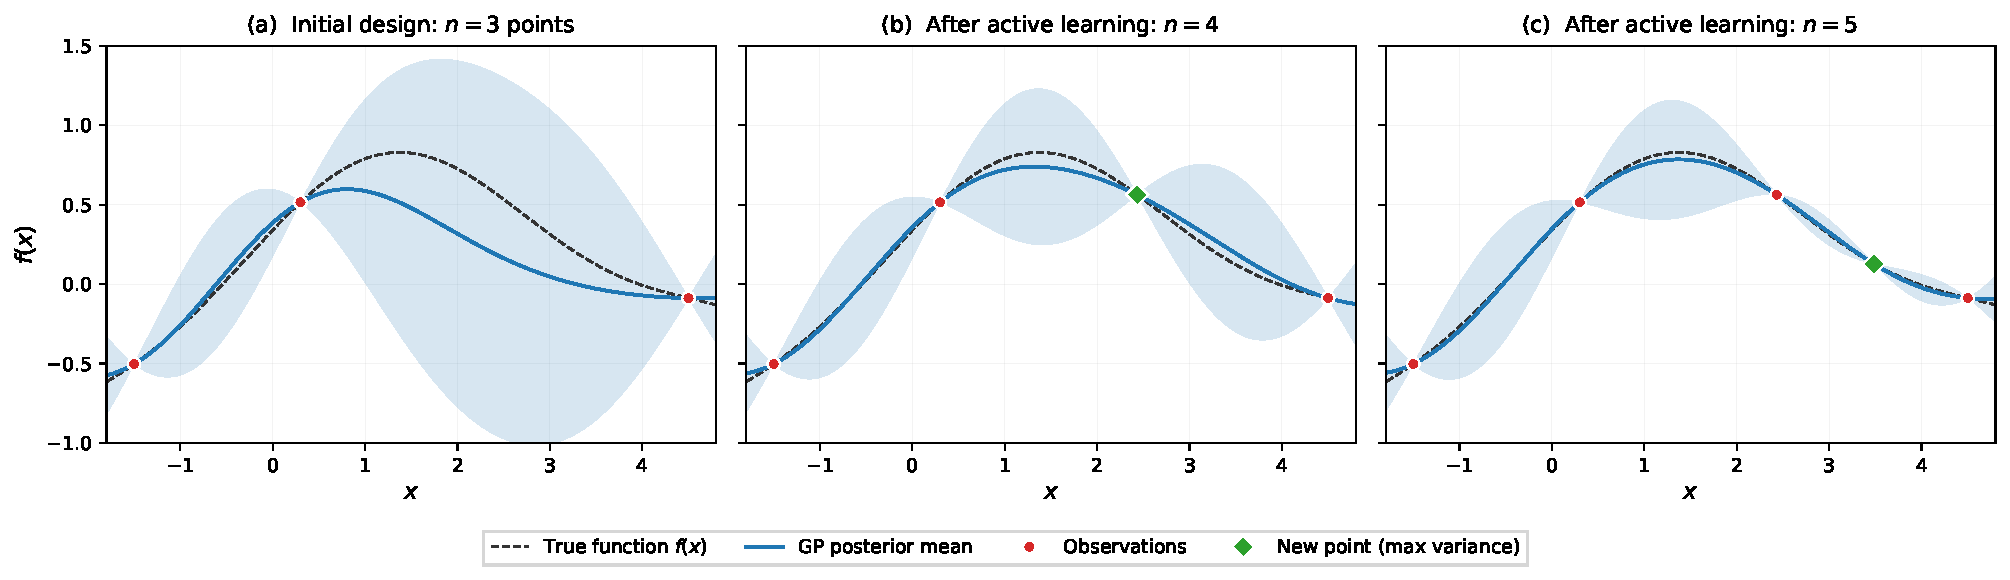
\includegraphics[width=0.95\textwidth]{gp_active_learning.pdf}
\end{center}

\vspace{-0.3cm}
{\footnotesize
\begin{itemize}\setlength{\itemsep}{0pt}\setlength{\parskip}{0pt}
  \item[\textbf{(a)}] 3 initial observations (red dots); GP posterior (blue) deviates in data-sparse regions with wide 95\% CI.
  \item[\textbf{(b)}] Acquisition function picks max-variance point (green diamond); posterior tightens locally.
  \item[\textbf{(c)}] Second iteration fills the remaining gap --- 5 points suffice to track the true function.
\end{itemize}
\vspace{-0.15cm}
\textbf{Key contrast with uniform:} BAL concentrates points where the function is hardest to approximate.}
\end{frame}

% --- Slide 38: Applications in Economics ---
\begin{frame}{BAL in Economics}
\begin{columns}[T]
\begin{column}{0.48\textwidth}
\begin{block}{Grid-free approximation}
BAL + GP $=$ grid-free adaptive sparse grids:
\begin{itemize}\setlength{\itemsep}{1pt}
  \item No structured grid needed
  \item Refinement via posterior variance
  \item Scales to $d \leq 10$
\end{itemize}
\end{block}
\end{column}
\begin{column}{0.48\textwidth}
\begin{block}{Applications}
\begin{itemize}\setlength{\itemsep}{1pt}
  \item \textbf{Optimal carbon tax}
  \item \textbf{Dynamic incentives} (kinks)
  \item \textbf{Asset pricing} (moderate $d$)
\end{itemize}
\end{block}
\end{column}
\end{columns}

\vspace{0.3cm}
{\small References: Renner \& Scheidegger (2018); K\"ubler, Scheidegger \& Surbek (2025).}
\end{frame}

% --- Slide 39: BAL + GP for Surrogates ---
\begin{frame}[shrink=5]{Combining BAL and GP for Surrogates}
\begin{center}
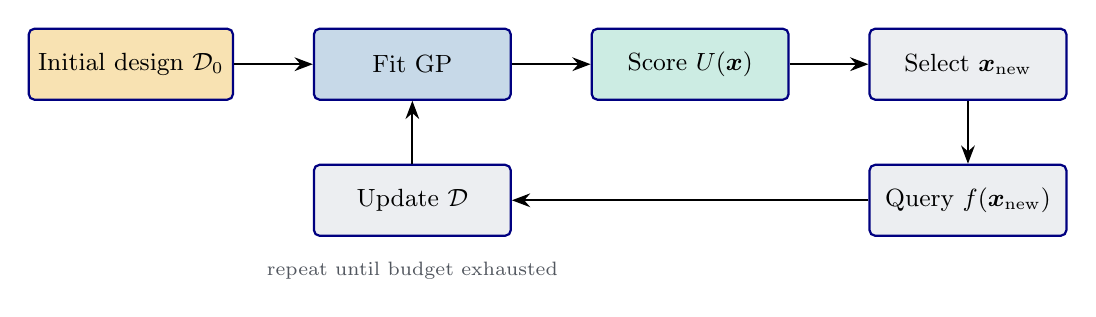
\begin{tikzpicture}[
    mlstep/.style={rectangle, draw=uzhblue, fill=uzhgreylight,
        minimum width=2.5cm, minimum height=0.9cm, font=\small,
        rounded corners=2pt, thick},
    >=Stealth
]
\node[mlstep, fill=softorange!30] (init) {Initial design $\mathcal{D}_0$};
\node[mlstep, right=1cm of init, fill=softblue!30] (gp) {Fit GP};
\node[mlstep, right=1cm of gp, fill=softgreen!20] (score) {Score $U(\x)$};
\node[mlstep, right=1cm of score] (select) {Select $\x_{\text{new}}$};
\node[mlstep, below=0.8cm of select] (query) {Query $f(\x_{\text{new}})$};
\node[mlstep, below=0.8cm of gp] (update) {Update $\mathcal{D}$};

\draw[->, thick] (init) -- (gp);
\draw[->, thick] (gp) -- (score);
\draw[->, thick] (score) -- (select);
\draw[->, thick] (select) -- (query);
\draw[->, thick] (query) -- (update);
\draw[->, thick] (update) -- (gp);

\node[below=0.2cm of update, font=\scriptsize, text=uzhgreydark] {repeat until budget exhausted};
\end{tikzpicture}
\end{center}

\vspace{0.3cm}
\begin{block}{Why this combination works}
\begin{itemize}
  \item \textbf{GP provides UQ:} posterior variance tells us where the approximation is uncertain.
  \item \textbf{BAL selects training points:} maximize information gain per model evaluation.
  \item \textbf{Surrogate = trained GP:} the same GP used for selection serves as the surrogate.
\end{itemize}
\end{block}

{\small Ideal for $d \leq 10$ when each model evaluation costs minutes to hours.}
\end{frame}

% --- Slide 40: Summary Part III ---
\begin{frame}{Summary: Bayesian Active Learning}
\begin{enumerate}
  \item \textbf{BAL} = principled data selection using GP uncertainty.
  \item \textbf{Score function} balances exploration (high $\sigma^2$) and exploitation (high $\mu$).
  \item \textbf{Faster convergence} than uniform sampling, especially for functions with kinks or local features.
  \item \textbf{Application:} surrogate construction for moderate-dimensional problems.
\end{enumerate}

\vspace{0.3cm}
\begin{block}{Hands-on}
\textbf{Notebook:} \texttt{02\_GP\_and\_BAL.ipynb} --- GP from scratch, scikit-learn GP, and BAL comparison.
\end{block}
\end{frame}

% ============================================================================
% PART IV: GAUSSIAN PROCESSES FOR DYNAMIC PROGRAMMING
% ============================================================================
\section{GPs for Dynamic Programming}

% --- Section Divider ---
\begin{frame}{}
\vfill
\begin{center}
{\Huge \textcolor{uzhblue}{\textbf{Part IV}}}\\[12pt]
{\LARGE Gaussian Processes for Dynamic Programming}\\[8pt]
{\small Based on: Scheidegger \& Bilionis (2019), \emph{J.\ Comput.\ Sci.}\ 33, 68--82.}
\end{center}
\vfill
\end{frame}

% --- Slide: What is Dynamic Programming? (simple intro) ---
\begin{frame}{What is Dynamic Programming?}
\small
\textbf{Dynamic programming} (DP) is the core method for solving \emphc{sequential decision problems} under uncertainty---the backbone of macro, finance, and structural IO.

\vspace{0.4em}
\begin{columns}[T]
\column{0.48\textwidth}
\textbf{The idea:} An agent makes decisions over time to maximize total discounted utility:
\[
V(\x_0) = \max \sum_{t=0}^{\infty} \beta^t\, r(\x_t, \xi_t)
\]
subject to $\x_{t+1} \sim F(\cdot \,|\, \x_t, \xi_t)$.

\vspace{0.3em}
\textbf{Bellman's principle of optimality:}
\[
V(\x) = \max_\xi \bigl\{ r(\x, \xi) + \beta\, \E{V(\x_{t+1})} \bigr\}
\]
Solve this \emphc{one equation} instead of the infinite-horizon problem.

\column{0.48\textwidth}
\textbf{Why DP matters:}
\begin{itemize}\itemsep1pt
    \item Asset pricing, consumption--savings
    \item Growth theory, capital accumulation
    \item Labor: job search, human capital
    \item Climate: optimal carbon taxation
\end{itemize}

\vspace{0.2em}
\textbf{Challenge:} Bellman equation on a \emphc{high-dimensional state space}---the curse of dimensionality.
\end{columns}
\end{frame}

% --- Slide: The Stochastic Growth Model ---
\begin{frame}{Example: The Stochastic Optimal Growth Model}
\small
Workhorse testbed for computational macro (cf.\ Days 2--3). Model with $D$ sectors:

\vspace{0.2em}
\begin{columns}[T]
\column{0.48\textwidth}
\begin{itemize}\itemsep0pt
    \item State: $\bm{k} = (k_1, \ldots, k_D)$
    \item Controls: consumption $\bm{c}$, labor $\bm{l}$, investment $\bm{i}$
    \item Production: $f(k_j, l_j) = A k_j^\psi l_j^{1-\psi}$
    \item Shocks: $\epsilon_{t,j} \sim \mathcal{N}(0, \sigma^2)$
    \item $k_{j}^+ = (1-\delta) k_j + i_j$
\end{itemize}

\vspace{0.2em}
$D$ ranges from 1 (textbook) to \emphc{500}.

\column{0.48\textwidth}
\textbf{Bellman equation:}
\[
V(\bm{k}) = \max_{\bm{c}, \bm{l}} \bigl\{ u(\bm{c}, \bm{l}) + \beta\, \E{V(\bm{k}^+)} \bigr\}
\]

\textbf{Challenge:} approximate $V$ on $\R^D$ at each VFI step. Grid methods fail for $D > 20$. \emphc{GPs as interpolation} $\Rightarrow$ arbitrary geometries, scales to 500D.
\end{columns}

\vspace{0.3em}
\begin{block}{Hands-on}
\small \texttt{04\_GP\_Value\_Function\_Iteration.ipynb} --- solves the $D=1$ case with GP-based VFI.
\end{block}
\end{frame}

% --- Slide: Key Idea ---
\begin{frame}{The Key Idea: GP as Value Function Surrogate}
\scriptsize
\begin{columns}[T]
\column{0.52\textwidth}
At each VFI step $s$:

\vspace{0.2em}
\begin{enumerate}\itemsep1pt
    \item Generate $n^s$ training inputs $\X$ in the state space
    \item Evaluate Bellman: $t_i^s = (TV^{s-1})(\x^{(i)})$
    \item Learn GP surrogate $V_{\text{surr}}$ from $\{\X, \bm{t}\}$
    \item Set $V^s = V_{\text{surr}}$ (posterior mean)
    \item Error: $\eta^s = \|V^s - V^{s-1}\|_\infty/\Delta_V$
\end{enumerate}

\vspace{0.2em}
GP posterior mean $\to$ next iterate; GP posterior \emphc{variance} $\to$ free uncertainty bounds at every step.

\column{0.45\textwidth}
\textbf{Why GPs instead of grids?}

\vspace{0.2em}
\begin{itemize}\itemsep1pt
    \item Work on \emphc{arbitrary geometries}---no tensor-product structure
    \item Training points \emphc{adaptively chosen}---concentrate near steep gradients
    \item Built-in \emphc{interpolation uncertainty}
    \item Non-converging points can be \emphc{discarded}---impossible with grids
\end{itemize}

\vspace{0.2em}
\begin{block}{Recall}
\tiny
Same GP posterior from Part~II, now applied iteratively inside a DP algorithm.
\end{block}
\end{columns}

\vspace{0.1em}
{\tiny \textbf{Origin:} GPDP — Deisenroth, Rasmussen \& Peters (2009, \emph{Neurocomputing}); economics/high-dim extension — Scheidegger \& Bilionis (2019, \emph{JoCS}).}
\end{frame}

% --- Slide: Algorithm ---
\begin{frame}[fragile]{Algorithm: ASGP Value Function Iteration}
\tiny
\begin{algorithmic}[1]
\STATE \textbf{Input:} Initial guess $V_{\text{next}}$, tolerance $\bar{\eta}$
\WHILE{$\eta > \bar{\eta}$}
    \STATE Generate $n^s$ training inputs $\X = \{\x^{(i)}\} \in [\underline{\bm{k}}, \bar{\bm{k}}]^D$
    \FOR{$\x^{(i)} \in \X$}
        \STATE Bellman target: $t_i = (TV_{\text{next}})(\x^{(i)})$; \quad policy: $\xi_j(\x^{(i)}) \in \argmax TV(\x^{(i)})$
    \ENDFOR
    \STATE Learn surrogate $V_{\text{surr}}$ with ASGP (or GP) from $\{\X, \bm{t}\}$
    \STATE Error: $\eta = \|V_{\text{surr}} - V_{\text{next}}\|_\infty$; \quad $V_{\text{next}} \leftarrow V_{\text{surr}}$
\ENDWHILE
\STATE \textbf{Output:} $V$, policy functions $\xi^* = (\xi_1^*, \ldots, \xi_{3D}^*)$
\end{algorithmic}

\vspace{0.3em}
{\scriptsize \textbf{Key:} Training set $\X$ can be \emphc{adaptively steered}---non-converging points excluded, new points added. Impossible with grids.}
\end{frame}

% --- New slide: Cheap BAL inside the VFI loop ---
\begin{frame}{Cheap BAL Inside the VFI Loop}
\textbf{Goal of acquisition.} Uniform interpolation accuracy of $V$, not optimization $\Rightarrow$ pure exploration.

\medskip
\textbf{Acquisition function.} Posterior standard deviation only:
\[
\x^{\text{next}} \in \argmax_{\x \in \mathcal{X}^{\text{cand}}} \sigma_{\text{GP}}^s(\x)
\quad \text{(no UCB, no EI).}
\]

\medskip
\textbf{Recipe.}
\begin{itemize}\itemsep0pt
  \item Every $N$ VFI iterations, score a Latin-hypercube candidate set
  \item Pick top $n_{\text{add}}$ by $\sigma_{\text{GP}}$, with min-spacing constraint to avoid clustering
  \item Evaluate Bellman operator at new points (parallel) and append to $\mathcal{D}^s$
\end{itemize}

\medskip
\textbf{Why pure exploration here.} A UCB-style acquisition would chase high-value states; we instead want $\sigma_{\text{GP}}$ small \emphc{everywhere} so the approximate Bellman operator stays close to a contraction.

\medskip
{\scriptsize Notebook 04 ($N=12$, $n_{\text{add}}=2$): active design beats naive LHS on both Bellman residual and LOO-RMSE.}
\end{frame}

% --- Slide: Active Subspaces ---
\begin{frame}{Active Subspaces: Breaking the Curse of Dimensionality}
\scriptsize
Standard GPs fail for $D \gtrsim 10$ (Euclidean distance uninformative). \emphc{Active Subspaces} (AS) find a low-dim manifold of maximal response variation.

\vspace{0.2em}
\begin{columns}[T]
\column{0.48\textwidth}
\textbf{Idea:} $f(\x) \approx h(\W^T\x)$, $\W \in \R^{D \times d}$, $d \ll D$.

\vspace{0.2em}
\textbf{Finding $\W$:}
\begin{enumerate}\itemsep0pt
    \item Collect gradients $\bm{g}^{(i)} = \nabla f(\x^{(i)})$
    \item $\bm{C}_N = \frac{1}{N}\sum \bm{g}^{(i)} (\bm{g}^{(i)})^T$
    \item SVD: $\bm{C}_N = \bm{V}\bm{\Lambda}\bm{V}^T$; find \emphc{sharp drop} in $\lambda_i$
    \item $\W = [\bm{v}_1, \ldots, \bm{v}_d]$ (top $d$ eigenvectors)
\end{enumerate}

\column{0.48\textwidth}
\textbf{The ASGP pipeline:}

\vspace{0.3em}
\begin{center}
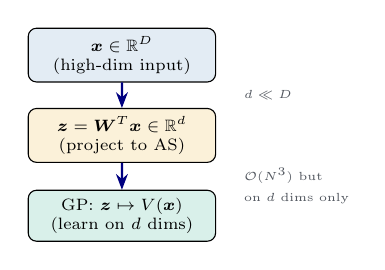
\begin{tikzpicture}[
    arr/.style={-{Stealth[length=2mm]}, thick, uzhblue},
    box/.style={draw, rounded corners=3pt, minimum width=2.8cm,
                minimum height=0.65cm, align=center, font=\scriptsize},
    scale=0.85, transform shape
]
    \node[box, fill=softblue!15] (hi) at (0,3) {$\x \in \R^D$\\(high-dim input)};
    \node[box, fill=softorange!15] (proj) at (0,1.8) {$\z = \W^T\x \in \R^d$\\(project to AS)};
    \node[box, fill=softgreen!15] (gp) at (0,0.6) {GP: $\z \mapsto V(\x)$\\(learn on $d$ dims)};
    \draw[arr] (hi) -- (proj);
    \draw[arr] (proj) -- (gp);
    \node[font=\tiny, text=uzhgreydark, anchor=west] at (1.7,2.4) {$d \ll D$};
    \node[font=\tiny, text=uzhgreydark, anchor=west] at (1.7,1.2) {$\mathcal{O}(N^3)$ but};
    \node[font=\tiny, text=uzhgreydark, anchor=west] at (1.7,0.85) {on $d$ dims only};
\end{tikzpicture}
\end{center}

\vspace{0.2em}
In the growth model, AS dim is typically $d = 1$, even when $D = 500$ $\Rightarrow$ \emphc{tractable}.
\end{columns}

\vspace{0.1em}
{\tiny \textbf{Hands-on:} \texttt{05\_Active\_Subspace\_2D}, \texttt{06\_..\_10D}, \texttt{07\_..\_Nonlinear} --- AS construction and ASGP vs GP comparison.}
\end{frame}

% --- Slide: When linear AS breaks ---
\begin{frame}{When the Active Manifold is Curved}
\scriptsize
Linear AS assumes the important directions are \emphc{linear} combinations of inputs: $f(\x) \approx h(\W^T \x)$.  If $f$ depends on a \emphc{nonlinear aggregate} of its inputs, the linear projection has to carry every direction that enters the aggregate -- not the aggregate itself.

\vspace{0.3em}
\begin{columns}[T]
\column{0.48\textwidth}
\textbf{Radial-ridge example} ($D = 20$):
\[
 y(\xi) \;=\; \exp\!\Bigl(-\bigl[(w_1^\top\xi)^2 + (w_2^\top\xi)^2\bigr]\Bigr).
\]
\begin{itemize}\itemsep0pt
  \item $C = \E[\nabla y\, \nabla y^\top]$ has \emphc{two} nonzero eigenvalues.
  \item Linear AS must pick $d_{\mathrm{lin}} = 2$.
  \item Yet the true intrinsic coordinate is the \emphc{scalar} $r^2 = (w_1^\top\xi)^2 + (w_2^\top\xi)^2$ -- one dimension.
\end{itemize}

\vspace{0.2em}
\textbf{Symptoms of curvature:}
\begin{itemize}\itemsep0pt
  \item Spectral gap ambiguous; $\lambda_i$ drops slowly.
  \item ASGP accuracy plateaus early as $d$ grows.
  \item Physics suggests thresholds, ridges, radial coords.
\end{itemize}

\column{0.48\textwidth}
\begin{center}
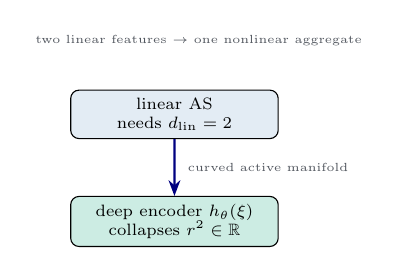
\begin{tikzpicture}[
    box/.style={draw, rounded corners=3pt, minimum width=3.1cm,
                minimum height=0.6cm, align=center, font=\scriptsize},
    arr/.style={-{Stealth[length=2mm]}, thick, uzhblue},
    scale=0.85, transform shape
]
    \node[box, fill=softblue!15]   (lin) at (0, 2.2) {linear AS\\needs $d_{\mathrm{lin}} = 2$};
    \node[box, fill=softgreen!20]  (nl)  at (0, 0.6) {deep encoder $h_\theta(\xi)$\\collapses $r^2 \in \R$};
    \draw[arr] (lin) -- node[right=2pt, font=\tiny, text=uzhgreydark]{curved active manifold} (nl);
    \node[font=\tiny, text=uzhgreydark, anchor=west] at (-2.2, 3.3) {two linear features $\to$ one nonlinear aggregate};
\end{tikzpicture}
\end{center}

\vspace{0.2em}
\textbf{Fix:} replace the linear projection $\W^T \x$ by a \emphc{learned nonlinear encoder} and jointly train a link function (Tripathy \& Bilionis, 2018).
\end{columns}

\vspace{0.1em}
{\tiny \textbf{Hands-on:} \texttt{09\_Deep\_Active\_Subspace\_Ridge} -- validates that deep AS recovers $d_{\mathrm{nl}} = 1$ on the radial ridge.}
\end{frame}

% --- Slide: Deep AS (Tripathy-Bilionis) ---
\begin{frame}{Deep Active Subspaces (Tripathy \& Bilionis, 2018)}
\scriptsize
Parametrize the surrogate as $\hat f(\xi) = g\bigl(h_\theta(\xi)\bigr)$, with \emphc{encoder} $h_\theta: \R^D \to \R^d$ and \emphc{link} $g_\theta: \R^d \to \R$ both small MLPs.  Setting $h_\theta(\xi) = U_m^\top \xi$ recovers the linear-AS ansatz, so the nonlinear encoder generalizes it.

\vspace{0.3em}
\begin{columns}[T]
\column{0.50\textwidth}
\textbf{Three design choices:}
\begin{enumerate}\itemsep1pt
  \item \textbf{Widths} decay exponentially
  $d_k = \lceil D \exp(\eta_{\mathrm{w}} k)\rceil$, $\eta_{\mathrm{w}} = \tfrac{1}{L}\log(d/D)$.
  \item \textbf{Swish activation} $\sigma(z) = z/(1 + e^{-z})$ (smooth, non-saturating).
  \item \textbf{Elastic-net loss}
  $\mathcal L = \tfrac{1}{N}\sum(\hat f - y_i)^2 + \lambda_1\|\theta\|_1 + \lambda_2\|\theta\|_2^2$.
\end{enumerate}

\vspace{0.3em}
\textbf{Gradient-free.} Learned from $(\xi_i, y_i)$ alone -- no $\nabla f$ samples, no orthogonality constraint.

\vspace{0.2em}
\textbf{Choosing $d$.} No spectral gap; use a \emphc{validation-MSE elbow} across $d = 1, 2, 3, \ldots$

\column{0.46\textwidth}
\begin{center}
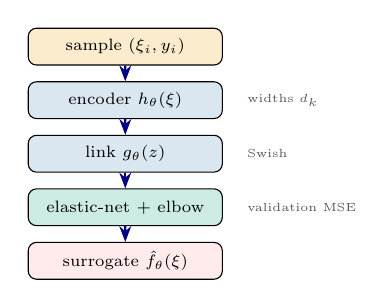
\begin{tikzpicture}[
    box/.style={draw, rounded corners=3pt, minimum width=2.9cm,
                minimum height=0.55cm, align=center, font=\scriptsize},
    arr/.style={-{Stealth[length=2mm]}, thick, uzhblue},
    scale=0.85, transform shape
]
    \node[box, fill=softorange!20] (sam)   at (0, 3.0) {sample $(\xi_i, y_i)$};
    \node[box, fill=softblue!20]   (enc)   at (0, 2.2) {encoder $h_\theta(\xi)$};
    \node[box, fill=softblue!20]   (lnk)   at (0, 1.4) {link $g_\theta(z)$};
    \node[box, fill=softgreen!20]  (eln)   at (0, 0.6) {elastic-net + elbow};
    \node[box, fill=red!8]         (sur)   at (0,-0.2) {surrogate $\hat f_\theta(\xi)$};
    \draw[arr] (sam) -- (enc);
    \draw[arr] (enc) -- (lnk);
    \draw[arr] (lnk) -- (eln);
    \draw[arr] (eln) -- (sur);
    \node[font=\tiny, text=uzhgreydark, anchor=west] at (1.7, 2.2) {widths $d_k$};
    \node[font=\tiny, text=uzhgreydark, anchor=west] at (1.7, 1.4) {Swish};
    \node[font=\tiny, text=uzhgreydark, anchor=west] at (1.7, 0.6) {validation MSE};
\end{tikzpicture}
\end{center}
\end{columns}

\vspace{0.1em}
{\tiny \textbf{Rule of thumb:} fit linear AS first; escalate to deep AS when (i) no gradients, (ii) ambiguous spectral gap, or (iii) $D \gg 10$ with curved manifold. \textbf{Hands-on:} \texttt{09\_..\_Ridge} (curved wins), \texttt{10\_..\_Borehole} (linear wins).}
\end{frame}

% --- Slide: Deep AS -- training recipe ---
\begin{frame}{Recipe: Fit a Deep Active Subspace}
\scriptsize
Self-contained recipe for the Tripathy-Bilionis architecture. All steps rely only on $(\xi_i, y_i)$ pairs -- no gradients, no Stiefel constraint, no kernel choice.

\vspace{0.2em}
\begin{columns}[T]
\column{0.54\textwidth}
\textbf{Algorithm.}
\begin{enumerate}\itemsep1pt
  \item \textbf{Sample} $(\xi_i, y_i)_{i=1}^N$; $80/20$ train/val split.
  \item \textbf{Standardize} inputs (unit variance), center outputs.
  \item For $d \in \{1, 2, 3, \ldots\}$:
    encoder $h_\theta\!: \R^D\!\to\!\R^d$ with widths $d_k = \lceil D e^{\eta_{\mathrm{w}} k}\rceil$, link $g_\theta\!: \R^d\!\to\!\R$ ($16$--$32$ units); train on
    $\mathcal L = \text{MSE}(\hat f, y) + \lambda_1\|\theta\|_1 + \lambda_2\|\theta\|_2^2$ with Adam + cosine LR.
  \item \textbf{Pick} $d$ at the \emph{validation-MSE elbow}.
  \item \textbf{Deploy}: $\hat f_\theta$ is the surrogate; $h_\theta(\xi)\!\in\!\R^d$ is a nonlinear \emphc{active coordinate} usable downstream (GP, sensitivity, optimization).
\end{enumerate}

\column{0.42\textwidth}
\textbf{Default hyperparameters:}
\vspace{0.1em}
\begin{center}
\renewcommand{\arraystretch}{1.05}
\tiny
\begin{tabular}{l l}
\toprule
encoder depth $L$ & $3$ \\
link hidden units & $16$--$32$ \\
activation & Swish ($\gamma = 1$) \\
optimizer & Adam, lr $5{\times}10^{-3}$ \\
schedule & cosine, $10^3$--$2{\cdot}10^3$ eps \\
$\lambda_1, \lambda_2$ & $10^{-5},\,10^{-4}$ \\
batch size & full batch if $N \lesssim 10^4$ \\
\bottomrule
\end{tabular}
\end{center}

\vspace{0.1em}
{\tiny \textbf{Samples:} $N \!\approx\! 50\,d_{\mathrm{nl}}$ to find the bottleneck, $\approx 200\,d_{\mathrm{nl}}$ for deployment.}
\end{columns}

\vspace{0.1em}
{\tiny \textbf{Sanity checks:} (i) validation curve monotone-then-flat in $d$; (ii) scatter of $h_\theta(\xi_i)$ vs.\ the first linear-AS coordinate shows whether the encoder has actually gone \emph{nonlinear}.}
\end{frame}

% --- Slide: Deep AS -- the elbow ---
\begin{frame}[shrink=5]{Reading the Validation-MSE Elbow}
\scriptsize
The spectral-gap heuristic of linear AS has no direct analogue for a neural encoder.  Tripathy \& Bilionis (2018) replace it by a \emphc{validation-MSE elbow}: train several latent dimensions and stop when extra capacity stops reducing held-out error.

\vspace{0.3em}
\begin{columns}[T]
\column{0.46\textwidth}
\textbf{How to read it.}
\begin{itemize}\itemsep1pt
  \item Plateau for $d \ge d_{\mathrm{nl}}$ $\Rightarrow$ intrinsic dim reached.
  \item Linear AS needs $d_{\mathrm{lin}} \ge d_{\mathrm{nl}}$ whenever the aggregate is nonlinear: the elbow sits \emphc{below} the spectral gap.
  \item If curves cross (as on the borehole) the function is nearly a ridge and linear AS + polynomial link is more data-efficient.
\end{itemize}

\vspace{0.2em}
\textbf{Three common shapes:}
\begin{itemize}\itemsep1pt
  \item \emphc{Sharp elbow at $d = 1$} -- classic radial / ridge target; deep AS wins.
  \item \emphc{Gradual decay} -- weak low-rank structure; more samples or richer encoder needed.
  \item \emphc{Flat} -- no low-dim structure; return to the original $D$-dimensional problem.
\end{itemize}

\column{0.50\textwidth}
\begin{center}
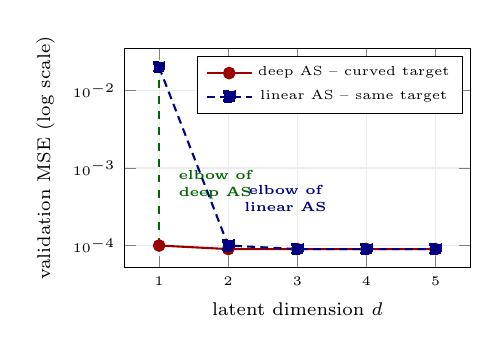
\begin{tikzpicture}[scale=0.95, transform shape]
\begin{axis}[
    width=6.2cm, height=4.5cm,
    xlabel={latent dimension $d$},
    ylabel={validation MSE (log scale)},
    ymode=log,
    xmin=0.5, xmax=5.5,
    xtick={1,2,3,4,5},
    ytick={1e-1,1e-2,1e-3,1e-4},
    grid=major, grid style={gray!15},
    legend style={font=\tiny, at={(0.98,0.97)}, anchor=north east},
    tick label style={font=\tiny},
    label style={font=\scriptsize},
]
\addplot[color=harvardcrimson, mark=*, thick]
  coordinates {(1,1e-4) (2,9e-5) (3,9e-5) (4,9e-5) (5,9e-5)};
\addlegendentry{deep AS -- curved target}
\addplot[color=uzhblue, mark=square*, thick, densely dashed]
  coordinates {(1,2e-2) (2,1e-4) (3,9e-5) (4,9e-5) (5,9e-5)};
\addlegendentry{linear AS -- same target}
\draw[dashed, darkgreen, thick]
  (axis cs:1,1e-4) -- (axis cs:1,2e-2);
\node[font=\tiny\bfseries, darkgreen, anchor=west]
  at (axis cs:1.15, 6e-4) {\shortstack{elbow of\\deep AS}};
\node[font=\tiny\bfseries, uzhblue, anchor=west]
  at (axis cs:2.1, 4e-4) {\shortstack{elbow of\\linear AS}};
\end{axis}
\end{tikzpicture}
\end{center}
{\tiny Stylized picture of the radial-ridge experiment (notebook \texttt{09}): deep AS flattens at $d = 1$, linear AS at $d = 2$.}
\end{columns}

\vspace{0.1em}
{\tiny \textbf{Operational test:} a drop of $<\!2\times$ in validation MSE between $d$ and $d+1$ is \emphc{not} worth paying the extra latent dimension for in most applications.}
\end{frame}

% --- Slide: Parallelization ---
\begin{frame}{Parallelization: Embarrassingly Parallel VFI}
\small
Bellman evaluations at $n^s$ training points are \emphc{independent} $\Rightarrow$ embarrassingly parallel.

\vspace{0.3em}
\begin{columns}[T]
\column{0.50\textwidth}
\textbf{MPI workflow:}
\begin{enumerate}\itemsep1pt
    \item \textbf{Broadcast} current $V_{\text{next}}$ to all workers
    \item \textbf{Evaluate:} each worker solves $n^s / n_{\text{cpu}}$ Bellman problems
    \item \textbf{Gather} training targets at master
    \item \textbf{Fit GP} surrogate (done once, centrally)
\end{enumerate}

\vspace{0.2em}
Communication cost negligible. Most time in parallelizable Bellman evaluations.

\column{0.47\textwidth}
\textbf{Scaling} (stochastic growth model):

\vspace{0.2em}
\scriptsize
\renewcommand{\arraystretch}{1.1}
\begin{tabular}{r r r}
\toprule
$D$ & Nodes & Total CPU h \\
\midrule
10 & 1 & 0.01 h \\
50 & 10 & 0.5 h \\
100 & 20 & 4 h \\
200 & 50 & 30 h \\
500 & 100 & $\sim$3700 h \\
\bottomrule
\end{tabular}

\vspace{0.3em}
\small
CPU time grows \emphc{sub-exponentially} ($<$2 days wall-clock for 500D with 100 nodes).
\end{columns}
\end{frame}

% --- Slide: Results ---
\begin{frame}[shrink=5]{Results: 1D to 500D Stochastic Growth}
\small
\begin{columns}[T]
\column{0.48\textwidth}
\textbf{Key results} (see Figs.~1--5 in the paper):
\begin{itemize}\itemsep3pt
    \item \textbf{1D:} Convergence in $\sim$70 VFI iterations; error $10^{-1} \to 10^{-5}$; GP CI bands negligible with just 10 training points
    \item \textbf{10D:} GP alone works; ASGP ($d=1$) equally accurate
    \item \textbf{50--500D:} ASGP converges to $10^{-4}$ normalized error; all dimensions converge in $\sim$70 iterations
\end{itemize}

\column{0.48\textwidth}
\textbf{Why this works:}
\begin{itemize}\itemsep3pt
    \item Active Subspace dimension is $d=1$ even for $D=500$ $\Rightarrow$ GP operates on 1D projected input
    \item Training set adaptively steered (drop non-converging points)
    \item Grid methods (Smolyak) cannot handle $D > 100$; ASGP \emphc{avoids the explicit grid-based curse} (does not eliminate all high-$d$ costs)
\end{itemize}
\end{columns}

\vspace{0.4em}
\begin{block}{Hands-on}
\textbf{Notebook:} \texttt{04\_GP\_Value\_Function\_Iteration.ipynb} --- solves the 1D growth model with GP-based VFI using scikit-learn. Shows convergence, value function with CI bands, and policy functions.
\end{block}
\end{frame}

% --- New slide: 2D GP-VFI in action ---
\begin{frame}{2D GP-VFI in Action}
\centering
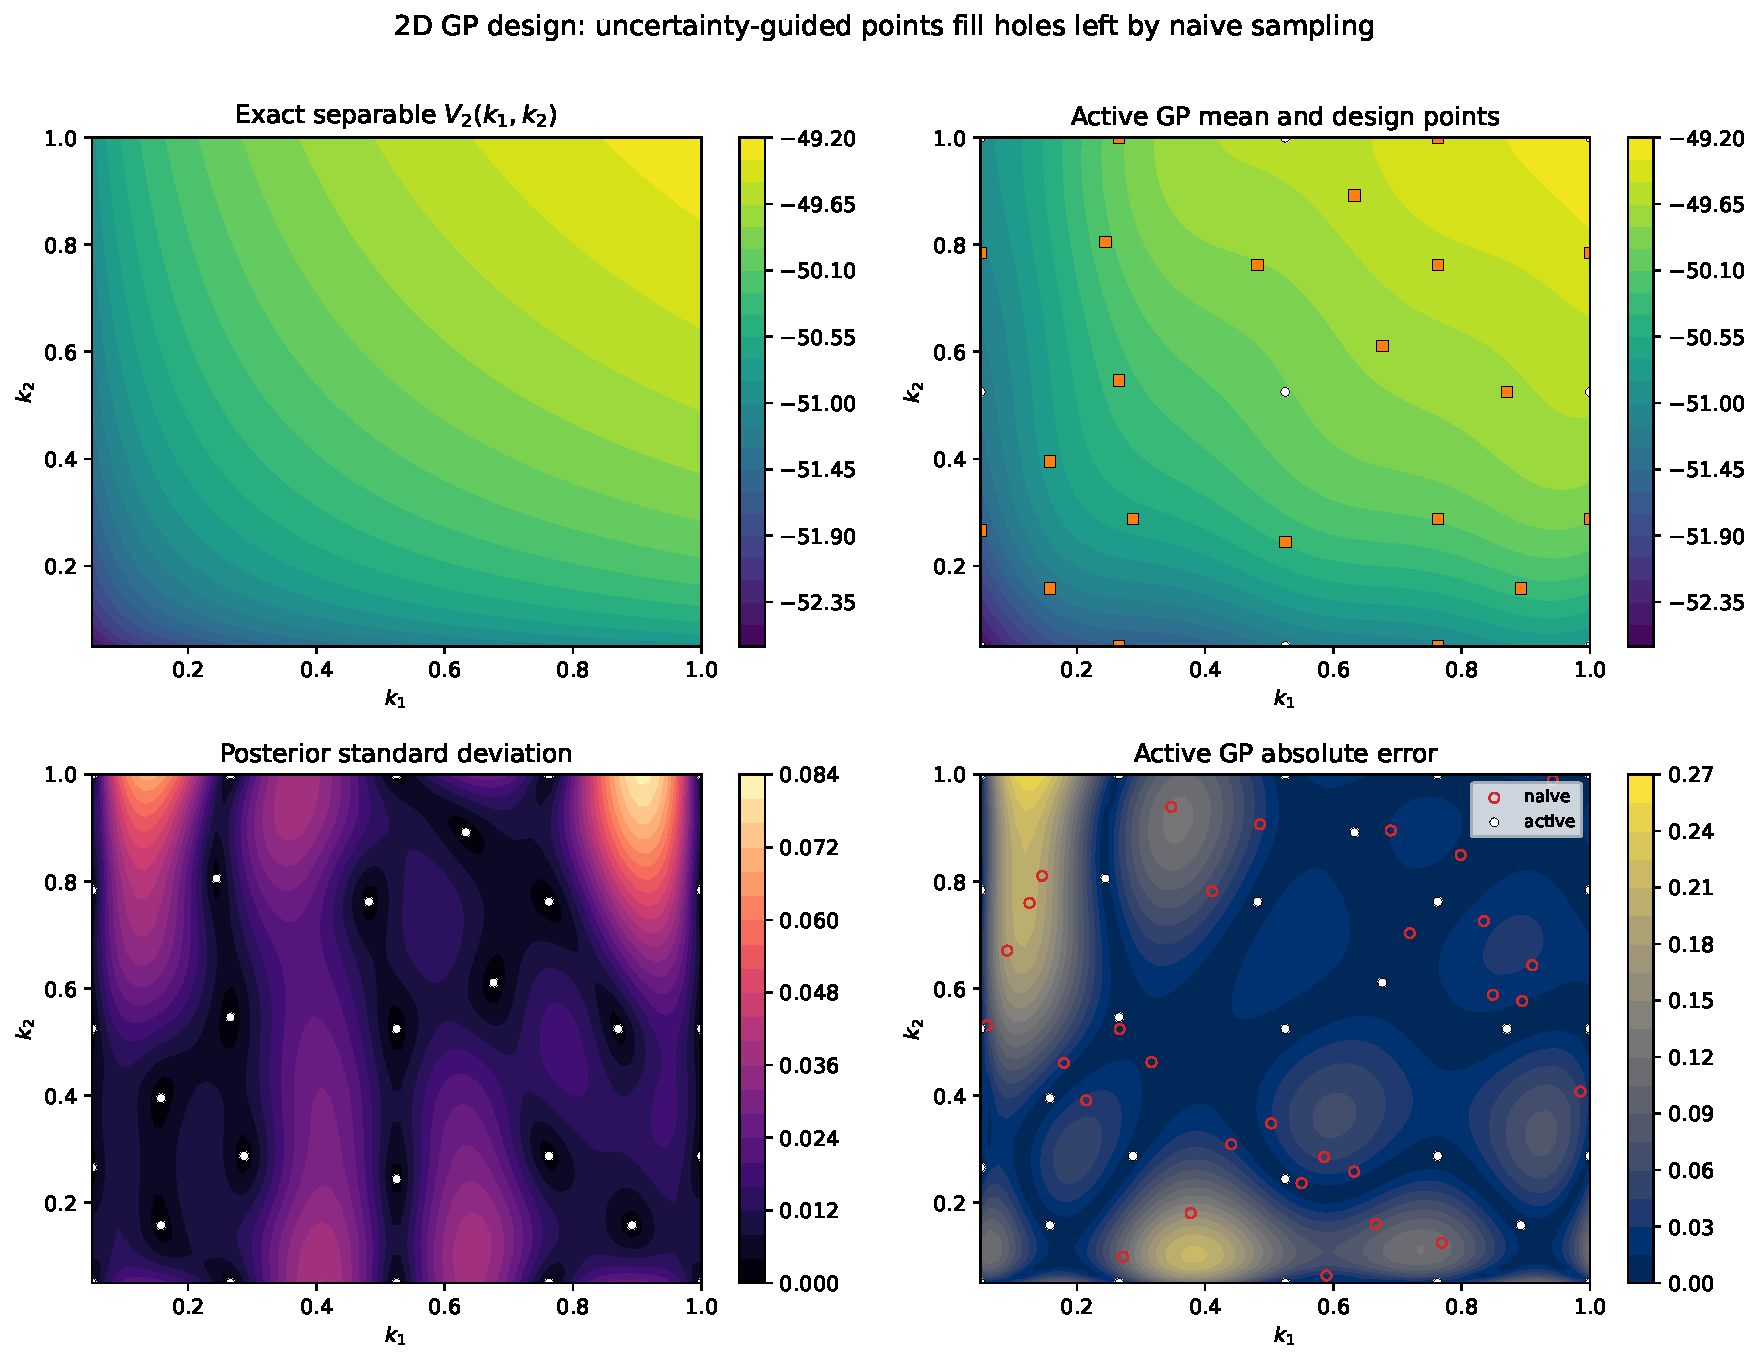
\includegraphics[height=0.72\textheight,keepaspectratio]{fig/gp_vfi_2d_active_benchmark.pdf}

\smallskip
{\scriptsize Separable benchmark $V_2(k_1,k_2) = V^*(k_1) + V^*(k_2)$ with $\delta = 1$ closed form. Active design places points where $\sigma_{\text{GP}}$ is largest. (Notebook 04, cell~25.)}
\end{frame}

% --- Finger Exercise: GP-VFI ---
\begin{frame}{\exercisepause{} Finger Exercise: One Step of GP-Based VFI}
\begin{exampleblock}{Exercise}
Consider a 1D growth model with $V(k) = \max_c \{ \log(c) + \beta\, V(k') \}$, $k' = k^{0.36} - c$, $\beta = 0.96$.  Suppose you have a GP trained on 3 points: $V(0.5) = -8.0$, $V(1.5) = -2.5$, $V(2.5) = 0.5$.
\begin{enumerate}
    \item At $k = 1.0$ (a new point not in the training set): the Bellman maximization yields $V^{\text{new}}(1.0) = -4.1$.  How does the GP posterior update when you add this observation?
    \item Does the GP posterior \emphc{variance} at $k = 1.0$ increase or decrease after adding this point?
    \item Why is it advantageous that training points can be added or removed freely, unlike grid-based methods?
\end{enumerate}
\end{exampleblock}
\end{frame}

\begin{frame}{Solution: One Step of GP-Based VFI}
\begin{block}{Answer}
\begin{enumerate}
    \item The GP is retrained on 4 points: $\{0.5, 1.0, 1.5, 2.5\}$.  The posterior mean $\mu(k)$ now interpolates through all 4 observations exactly (noiseless GP).  The posterior mean between existing points adjusts to accommodate the new observation.
    \item The posterior variance at $k = 1.0$ \emphc{decreases to zero} (the GP passes through the observation exactly).  Variance at nearby points also decreases.  Variance far from all training points remains large.
    \item \emphc{Flexibility:} If the Bellman operator at some point fails to converge (e.g., near a constraint), that point can simply be dropped.  On a grid, removing a point breaks the tensor-product structure.  This is a key advantage of GP-based VFI over grid-based methods.
\end{enumerate}
\end{block}
\end{frame}

% --- Slide: UQ and Ergodic Sets ---
\begin{frame}{UQ as a Byproduct \& Learning Ergodic Sets}
\scriptsize
\begin{columns}[T]
\column{0.48\textwidth}
\textbf{Uncertainty quantification:}

The GP posterior variance provides \emphc{free UQ} for the interpolated value function at every state point and VFI iteration. Policy uncertainty must be propagated through the maximization step.

\vspace{0.3em}
\textbf{Parameter uncertainty propagation:}
\begin{itemize}\itemsep1pt
    \item Add uncertain parameters as \emphc{pseudo-states}:\\
    $\tilde{S} = (\bm{k}, \gamma)$ where $\gamma \in [\underline{\gamma}, \bar{\gamma}]$
    \item Solve the model once on the extended state space
    \item Extract univariate effects: $\mathcal{M}_i(\chi_i) = \E{\mathcal{M}(\Theta) \mid \Theta_i = \chi_i}$
    \item Global sensitivity analysis (Sobol-style) in a \emphc{single computation}
\end{itemize}

\vspace{0.2em}
{\scriptsize This avoids the traditional approach of re-solving the model for each parameter value.}

\column{0.48\textwidth}
\textbf{Learning ergodic sets:}

Many economic models have \emphc{irregularly shaped} ergodic sets (ellipsoids, not hypercubes).

\vspace{0.3em}
\begin{enumerate}\itemsep2pt
    \item Solve model on a large domain initially
    \item Simulate the economy to generate capital paths $\{\bm{k}_t^+\}$
    \item Fit a \emphc{Bayesian Gaussian Mixture Model} to learn\\
    $\hat{\rho}_{\text{ergodic}}(\x)$
    \item Re-solve on the ergodic set only---sample training points from $\hat{\rho}_{\text{ergodic}}$ instead of the full hypercube
\end{enumerate}

\vspace{0.3em}
GPs handle this naturally: no grid structure to reconfigure. Training points can be placed \emphc{anywhere} in the state space.
\end{columns}
\end{frame}

% --- Slide: GPs vs DEQNs ---
\begin{frame}{GPs vs.\ DEQNs for Solving Dynamic Models}
Both are \emphc{complementary tools}---choose based on problem structure:

\vspace{0.3em}
\begin{center}
\scriptsize
\renewcommand{\arraystretch}{1.15}
\begin{tabular}{p{2.8cm} p{3.8cm} p{3.8cm}}
\toprule
 & \textbf{GP / ASGP} & \textbf{DEQNs (Days 2--4)} \\
\midrule
Method & Value function iteration & Euler equation residuals \\
Dimensionality & Up to $\sim$500 (with AS) & $>$1000 feasible \\
UQ built-in & \textcolor{darkgreen}{\textbf{Value}} (GP variance) & \textcolor{darkred}{\textbf{No}} \\
Hardware & CPU clusters (MPI) & GPUs \\
Irregular domains & \textcolor{darkgreen}{\textbf{Yes}} & \textcolor{darkgreen}{\textbf{Yes}} \\
Sensitivity analysis & Cheap with pseudo-states & Pseudo-states or re-training \\
\bottomrule
\end{tabular}
\end{center}

\vspace{0.3em}
\small
\textbf{Use GPs} when effective dimension is moderate and you need value-function UQ or sensitivity analysis.

\textbf{Use DEQNs} when $D$ is very large, you have GPU access, or you need complicated market-clearing conditions.
\end{frame}

% --- Slide: Summary of GP pipeline ---
\begin{frame}{Summary: The Full GP Pipeline for Economics}
The same GP machinery, applied at \emphc{increasing levels of ambition}:

\vspace{0.4em}
\begin{center}
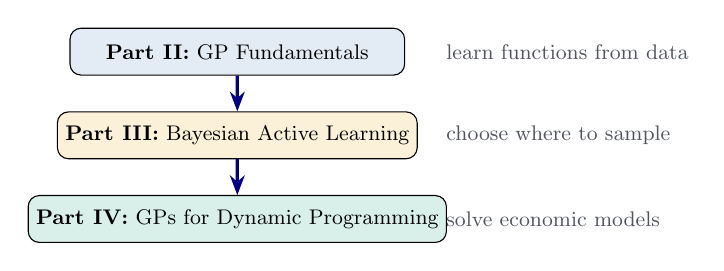
\begin{tikzpicture}[
    box/.style={draw, rounded corners=4pt, minimum width=5cm,
                minimum height=0.7cm, align=center, font=\small},
    arr/.style={-{Stealth[length=2.5mm]}, very thick, uzhblue},
    scale=0.85, transform shape
]
    \node[box, fill=softblue!15] (gp) at (0,2.5) {\textbf{Part II:} GP Fundamentals};
    \node[box, fill=softorange!15] (bal) at (0,1.25) {\textbf{Part III:} Bayesian Active Learning};
    \node[box, fill=softgreen!15] (dp) at (0,0) {\textbf{Part IV:} GPs for Dynamic Programming};

    \draw[arr] (gp) -- (bal);
    \draw[arr] (bal) -- (dp);

    \node[font=\small, text=uzhgreydark, anchor=west] at (3,2.5) {learn functions from data};
    \node[font=\small, text=uzhgreydark, anchor=west] at (3,1.25) {choose where to sample};
    \node[font=\small, text=uzhgreydark, anchor=west] at (3,0) {solve economic models};
\end{tikzpicture}
\end{center}

\vspace{0.4em}
{\small Reference: Scheidegger \& Bilionis (2019), ``Machine Learning for High-Dimensional Dynamic Stochastic Economies,'' \emph{J.\ Computational Science} 33, 68--82.}

\vspace{0.2em}
\begin{block}{Hands-on}
\small \textbf{Notebook:} \texttt{04\_GP\_Value\_Function\_Iteration.ipynb} (in \texttt{day7/code/}).
\end{block}
\end{frame}

% ============================================================================
% PART V: SUMMARY & OUTLOOK
% ============================================================================
\section{Summary \& Outlook}

% --- Slide: Day 2 Recap ---
\begin{frame}{Recap: The Computational Toolbox}
\small
\begin{columns}[T]
\begin{column}{0.24\textwidth}
\begin{block}{\small PINNs}
\scriptsize
\begin{itemize}\itemsep0pt
  \item Continuous-time PDEs
  \item Physics loss
  \item Mesh-free
  \item HJB, Black--Scholes
\end{itemize}
\end{block}
\end{column}
\begin{column}{0.24\textwidth}
\begin{block}{\small Deep Surrogates}
\scriptsize
\begin{itemize}\itemsep0pt
  \item Discrete-time
  \item Pseudo-states
  \item Fast evaluation
  \item Estimation, UQ
\end{itemize}
\end{block}
\end{column}
\begin{column}{0.24\textwidth}
\begin{block}{\small GPs + BAL}
\scriptsize
\begin{itemize}\itemsep0pt
  \item Nonparametric
  \item Built-in UQ
  \item Active learning
  \item Moderate dim
\end{itemize}
\end{block}
\end{column}
\begin{column}{0.24\textwidth}
\begin{block}{\small ASGP + VFI}
\scriptsize
\begin{itemize}\itemsep0pt
  \item GP inside DP
  \item Active Subspaces
  \item Up to 500D
  \item Ergodic sets
\end{itemize}
\end{block}
\end{column}
\end{columns}

\vspace{0.3cm}
All four approaches are \emphc{complementary}: choose based on the problem structure, dimensionality, whether UQ is needed, and available hardware.
\end{frame}

% --- Slide 42: The Toolbox ---
\begin{frame}{The Toolbox: When to Use What}
\begin{center}
\scriptsize
\begin{tabular}{l l l}
\toprule
\textbf{Method} & \textbf{Best for} & \textbf{Key strength} \\
\midrule
\textbf{DEQN} & Discrete-time equilibrium models & Scales to high $d$, Euler eq.\ loss \\
\textbf{PINN} & Continuous-time PDEs/HJB & Mesh-free, physics-constrained \\
\textbf{Deep Surrogate} & Fast evaluation, estimation, UQ & Pseudo-states, autograd \\
\textbf{GP + BAL} & Moderate $d$, need UQ & Built-in uncertainty, active learning \\
\textbf{Deep Kernel} & Warped inputs + need UQ & Learned features + GP uncertainty \\
\bottomrule
\end{tabular}
\end{center}

\vspace{0.15cm}
\begin{block}{Decision heuristic}
\scriptsize
\begin{enumerate}
  \item Is it a continuous-time PDE? $\Rightarrow$ \textbf{PINN}.
  \item Do you need to re-evaluate for many parameter values? $\Rightarrow$ \textbf{Deep Surrogate}.
  \item Is $d \leq 10$ and you need UQ / active learning? $\Rightarrow$ \textbf{GP + BAL}.
  \item Is the latent structure smooth, but the raw input geometry is poor? $\Rightarrow$ \textbf{Deep Kernel}.
  \item Is it a discrete-time equilibrium model? $\Rightarrow$ \textbf{DEQN}.
\end{enumerate}
\end{block}
\end{frame}

% --- Slide 43: References & Questions ---
\begin{frame}[shrink=5]{References \& Resources}
\footnotesize
\textbf{Key papers:}
\begin{itemize}\itemsep0pt \parskip0pt
  \item Chen, Didisheim \& Scheidegger (2026). \emph{Deep Surrogates for Finance: With an Application to Option Pricing.} J.\ Financial Econ.
  \item Scheidegger \& Bilionis (2019). \emph{ML for High-Dim Dynamic Stochastic Economies.} J.\ Comput.\ Sci.
  \item K\"ubler, Scheidegger \& Surbek (2026). \emph{Using Machine Learning to Compute Constrained Optimal Carbon Tax Rules.} Forthcoming in \emph{JPE Macroeconomics}.
  \item Rasmussen \& Williams (2006). \emph{GP for ML.} MIT Press.
  \item Wilson et al.\ (2016). \emph{Deep Kernel Learning.} AISTATS.
\end{itemize}

\vspace{0.1cm}
{\tiny \textbf{Notebooks:} \texttt{01\_Surrogate\_Primer}, \texttt{02\_GP\_and\_BAL}, \texttt{03\_Structural\_Estimation\_BM}, \texttt{04\_GP\_Value\_Function\_Iteration}, \texttt{05--07\_Active\_Subspace} (2D, 10D, nonlinear), \texttt{08\_Deep\_Kernel\_Learning}, \texttt{09\_Deep\_Active\_Subspace\_Ridge}, \texttt{10\_Deep\_AS\_vs\_Linear\_AS\_Borehole}}

\vspace{0.15cm}
\textbf{GitHub:} \url{https://github.com/sischei/Deep_Learning_for_Solving_And_Estimating_Dynamic_Economic_Models}

\vspace{0.2cm}
\begin{center}
{\LARGE \emphc{Questions?}}
\end{center}
\end{frame}

\end{document}
